% Hypothesis summary writeup: the 15 most promising theses, with figures and animation storyboards.
% Build: cd writeup/hypothesis-summary-writeup && pdflatex hypothesis-summary-writeup && pdflatex hypothesis-summary-writeup
\documentclass[aps,pre,onecolumn,10pt,nofootinbib]{revtex4-2}
\usepackage{graphicx}
\usepackage{amsmath,amssymb}
\usepackage[T1]{fontenc}
\usepackage{xcolor}
\usepackage{tikz}
\usepackage[hidelinks]{hyperref}
\graphicspath{{../visuals/}{../../hypotheses/}}
% Claude spark, redrawn in TikZ (12 tapered rays). Usage: \claudespark  (inline, about 1em)
\definecolor{claudeorange}{HTML}{D97757}
\newcommand{\claudespark}{\tikz[baseline=-0.32em, x=0.52em, y=0.52em]{%
  \fill[claudeorange] (0,0) circle (0.30);
  \foreach \ang/\len/\w in {113.6/1.10/0.17, 80/0.99/0.15, 48/0.98/0.17, 11/1.0/0.15, -12/0.99/0.15, -39/1.0/0.14,
                             -59/0.97/0.15, -91/0.98/0.14, -121/0.98/0.15, -147/0.92/0.15, 177/1.0/0.15, 144/1.01/0.17}{
    \fill[claudeorange, rotate=\ang] (0,-\w) -- (\len-0.05,-0.6*\w) arc (-90:90:0.6*\w) -- (0,\w) -- cycle;}
}}

\newcommand{\cred}[1]{\,(credence~#1)}
\begin{document}
\title{Hypothesis summary writeup:\\ the 15 most promising theses about an LLM agent swarm}
\author{Claude Opus 5.5\,\claudespark}
\noaffiliation
\author{Vivian Rogers}
\noaffiliation
\date{\today}
\begin{abstract}
This document gives the 15 hypotheses with the highest estimated usefulness (EU), out of 132 tested on the AI Village record. EU is credence times value if true; two Claude judges, one blind, gave both numbers. Each entry has six parts: the question, the physical intuition, the measurement, the result, what it means for an operator, and the caveats. Each entry shows its figure. Seven entries also show a storyboard of their animation; the animation files are in \texttt{writeup/visuals/}. No claim here has passed a confirmation test on reserved data. Companion to the paper \texttt{writeup/paper/paper.pdf}.
\end{abstract}
\maketitle
\tableofcontents
\clearpage
% H44: erasure, re-acquisition and thrash. Sources: hypotheses/H44-erasure-reacquisition-thrash/{README.md, summary/content.tex, summary/meta.json};
% writeup/visuals/H44-context-wipe/{caption.tex, README.md}; interpretation/swarm-constants.json (ΔW_erase).
\section{H44: A context wipe costs output but does not heat the agent}

\textbf{The question:}
The scaffold wipes an agent's context window at a cap of 41 records (40 model calls) and keeps its memory.
Does the agent then thrash: re-read instead of produce, act more randomly and listen harder to the room?
How much output does each wipe cost?

\textbf{The intuition:}
Treat each model call as a spin with many states (write, run, read, look, talk, idle).
Three fields set its choice: a baseline field (the agent's habit with no task in mind), a room field and a task field in the context.
The wipe is a quench (a sudden change of a control parameter) that sets the task field to zero.
A \emph{field quench} shifts the mix of calls toward reading, and the task field then grows back over a few calls.
A \emph{temperature pulse} makes every choice more random, so the entropy of the call mix rises.
Linear response (a spin with a weak self-field follows an outside field more easily) predicts that a wiped agent follows the room more.

\textbf{What we measured:}
The data are nine regime-III goal periods outside the reserved data (G36--G51): 1.24M calls, 21{,}165 forced and 16{,}357 voluntary resets.
The thrash index $\Theta_c$ is the rise in the read share of non-write calls over calls $+1\ldots+5$.
It conditions on the agent and on the category of the previous call.
The write dip $\Omega$ compares writes over calls $+1\ldots+10$ with calls $-20\ldots-11$; DQ4 work commits give a second output measure.
The null is a set of pseudo-erasures: no-reset boundaries at call 21 or 31 of the same segments, at the same hours.
\emph{Scheduler field:} removed, because each event compares two sides of one reset within one agent-day.
\emph{External drive:} removed, because the cap, not the task state, times a forced wipe; its pre-trend equals the null band.
\emph{Shared model prior:} removed by the conditioning on agent and previous call; the effect holds in Anthropic, OpenAI and Google agents.
\emph{Common input:} the reply test is a difference-in-differences against pseudo-erasures, so a common response cancels.
\emph{Synthetic check:} three planted worlds (thrash, pure output dip, no effect) on real call skeletons.
At G51 counts the pipeline classifies all three correctly in 100\% of replicates.

\begin{figure}[h]
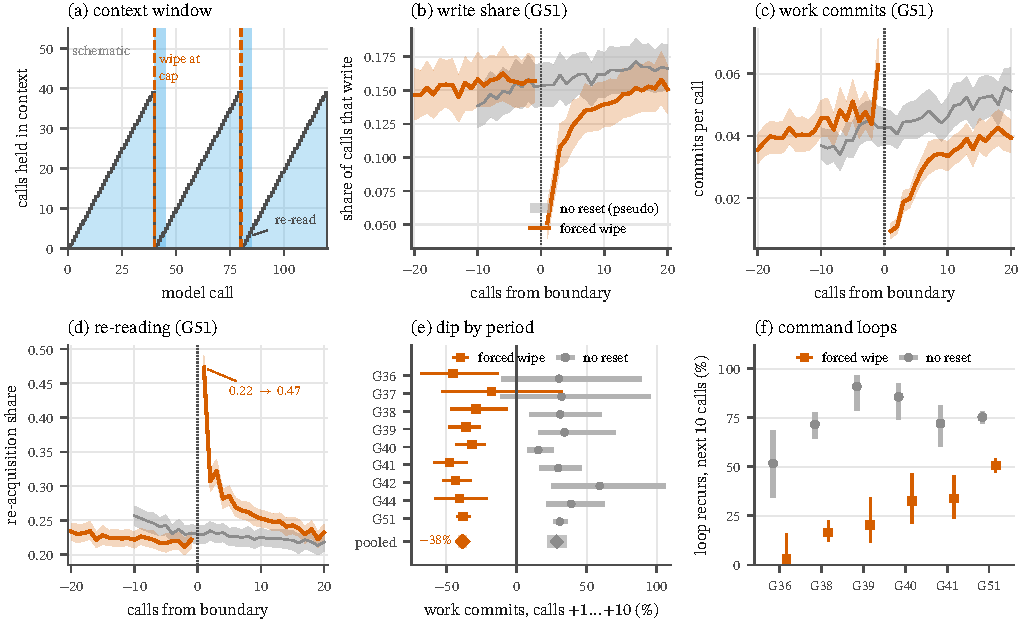
\includegraphics[width=\textwidth]{H44-context-wipe/fig.pdf}
\caption{What a forced context wipe does to one agent.
In G51 the share of re-reading calls doubles at the first call after the wipe. Writes and work commits dip for about three calls; the gray band is the no-reset null.
The lower panels show the work-commit dip in every period and the drop in command loops after a wipe.
Animation: \texttt{writeup/animations/H44-context-wipe.mp4}.}
\label{fig:int-H44}
\end{figure}
\begin{figure}[h]
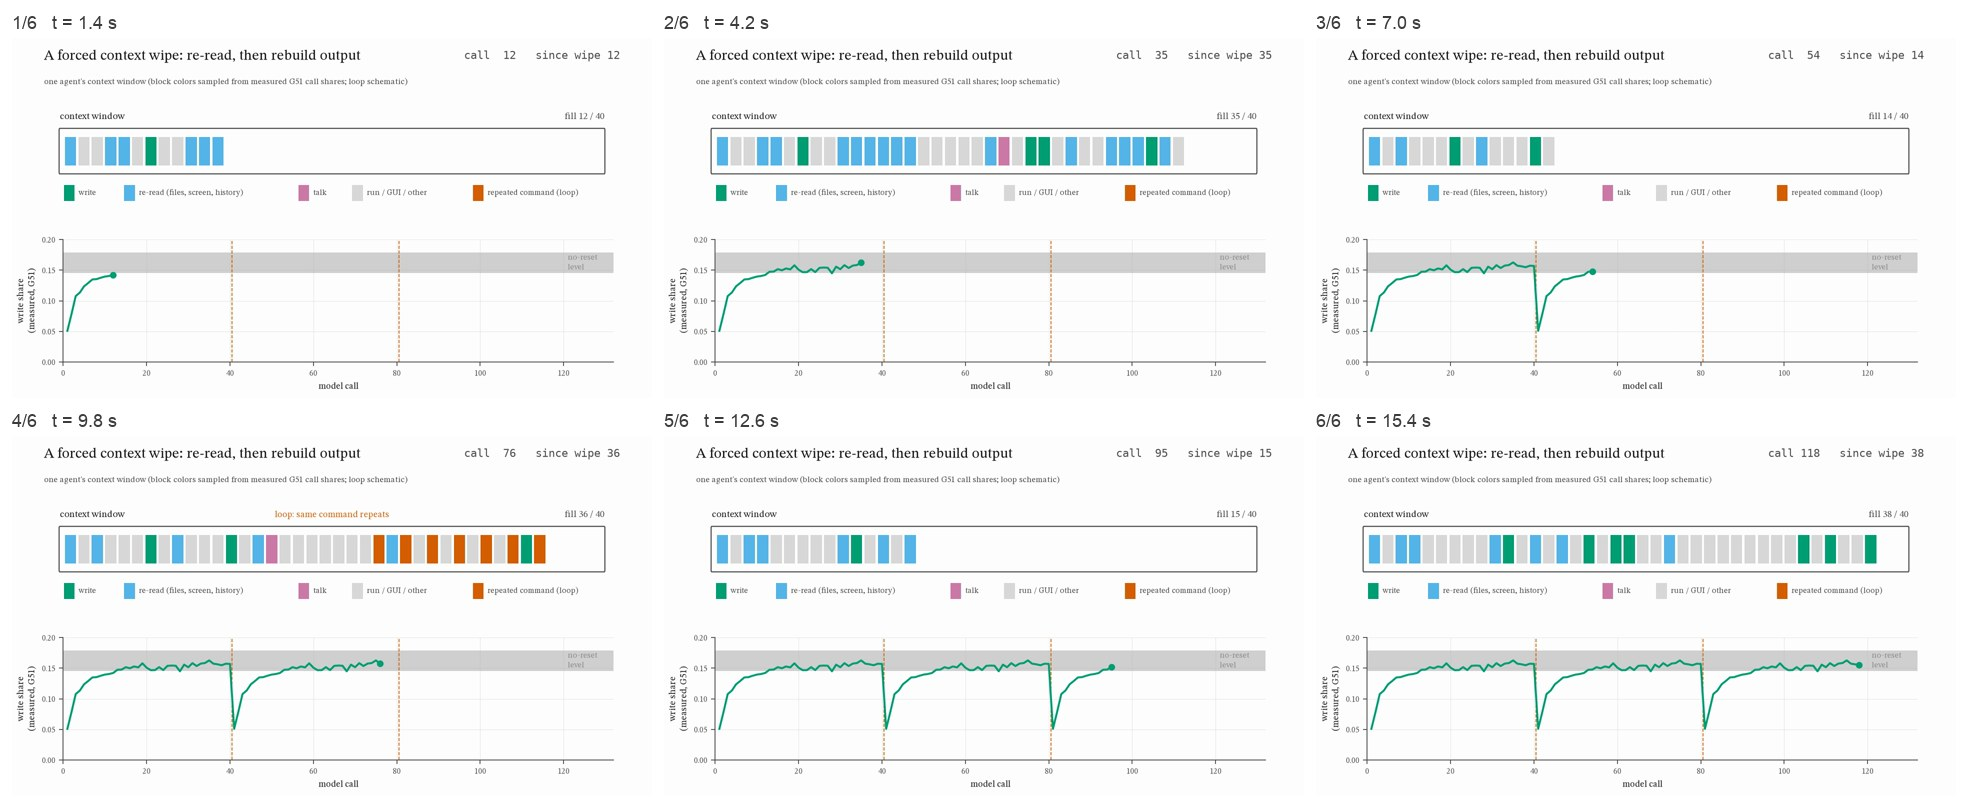
\includegraphics[width=0.9\textwidth]{storyboards/H44.jpg}
\caption{Animation storyboard: six frames of the animation, evenly spaced in time (frame number and time above each). The full animation is \texttt{writeup/animations/H44-context-wipe.mp4}.}
\end{figure}


\textbf{What we found:}
Re-acquisition is real; thrash is not.
In G51 the read share rises from 0.22 to 0.47 at the first call and relaxes over 5--7 calls.
$\Theta_c=+0.079$ [0.071, 0.086], positive in 9/9 periods; the null gives $-0.011$.
Writes fall 26\% [$-29$, $-23$] (8/9 periods), work commits fall 38\% [$-41$, $-35$], and real failures rise 1 point.
Per period the wipes cost 3.7--8.7\% of all write calls and 4.8--10.9\% of all work commits.
The entropy of the call mix \emph{falls} ($-0.027$): the agent reads in an orderly way, with no temperature pulse.
The reply rate to new room items does not change (rate ratio 0.97 [0.91, 1.04]; G51 0.90).
Coupling to items read before the wipe falls (ratio 0.60 [0.44, 0.81]).
A command loop recurs after a wipe in 16\% of cases, against 72\% without one (G38; pooled odds ratio 0.11 [0.05, 0.26], 7 periods).
Within regime III (nine periods), the claim ``a forced wipe triggers orderly re-reading, costs 4--11\% of output and breaks loops'' stands\cred{0.88}.
Its expected usefulness is EU~3.23 (value if true 3.67; three raters, one blind).

\textbf{What it means:}
For a scaffold builder, the cap length is a cost/benefit dial.
A 40-call cap costs about 4--11\% of output and breaks most command loops (odds ratio about 0.1).
Point a recovering agent at its working files.
An agent that first re-reads its files resumes writing 2.6 calls sooner than one that first looks at the screen.
Do not count on the memory note written at the wipe: its length has no effect on the dip ($\rho=-0.03$).
A freshly wiped agent is not easier for its peers to steer.

\textbf{Caveats:}
An unchecked regex classifier assigns the call categories, and it cannot separate GUI browsing from production.
Writes ramp up through each 40-call segment, so the size of the dip depends on the reference window.
The agent chooses what to re-read, so the ``files first'' result is observational.
The analysis runs about 12 statistics on nine periods with no correction; G37 has low power.
The fragile flag is not set, and no confirmation test on reserved goal periods has run.

% H50: field vs coupling from transfer lags. Sources: hypotheses/H50-field-vs-coupling-transfer-lag/{README.md, summary/content.tex, summary/meta.json};
% writeup/visuals/H50-field-vs-coupling-transfer-lag/{caption.tex, README.md}; interpretation/swarm-constants.json (J1 named vs unnamed).
\section{H50: Activity moves with the scheduler; talk moves one read-out call at a time}

\textbf{The question:}
When agents co-move, does a common input hit all of them (a field), or do they read each other (a coupling)? Can the lag tell?

\textbf{The intuition:}
Agents act only at model calls.
A field, for example the runner's daily start, reaches every agent at its next call.
So all agents respond within about one call cycle: the field has zero relative lag.
A coupling must pass through a message.
The message enters a recipient's context only at its next call, the read-out call.
So coupling lags come in whole call cycles, or hops.
Hop 0 is the call already in flight, which cannot see the message; hop 1 is the read-out call.
The test is a regression discontinuity: it compares calls that start just after a message with calls that start just before it.

\textbf{What we measured:}
The read-out jump $J_1$ is the extra chance that a recipient's hop-1 call is a talk call, minus a shifted-time placebo.
It uses the DQ1 context ledger, which records which call received which message.
The analysis also fits impulse responses (the response over time to one input) for day starts, pauses, human messages, nudges and platform errors.
It then splits co-movement into a field part and a coupling part.
It covers 71 units in 35 goal periods outside the reserved data, in all three regimes, plus 4 period-native tests.
\emph{Scheduler field:} measured as an input against a shifted-input null, with an all-running-window variant.
\emph{External drive:} human messages, nudges, operator bookends and errors enter as fields.
Goal kickoffs are not among the inputs, so this impostor is only partly removed.
\emph{Shared model prior:} not relevant, because a family prior cannot make a step at the read-out call.
\emph{Common input:} removed by the comparison of the in-flight call with the read-out call; the in-flight side is not raised.
\emph{Synthetic check:} 15 planted scenarios $\times$ 5 seeds on real village schedules.
$J_1$ recovers planted coupling with a bias of $-2$ to $-17\%$ in regime III.
It reads zero for fields and slow common drives, and it finds a planted 2-hop dead time as onset at hop 3.
It goes negative for a coupling that acts within the call in flight.
False positives occur in 3/35 null seeds.

\begin{figure}[h]
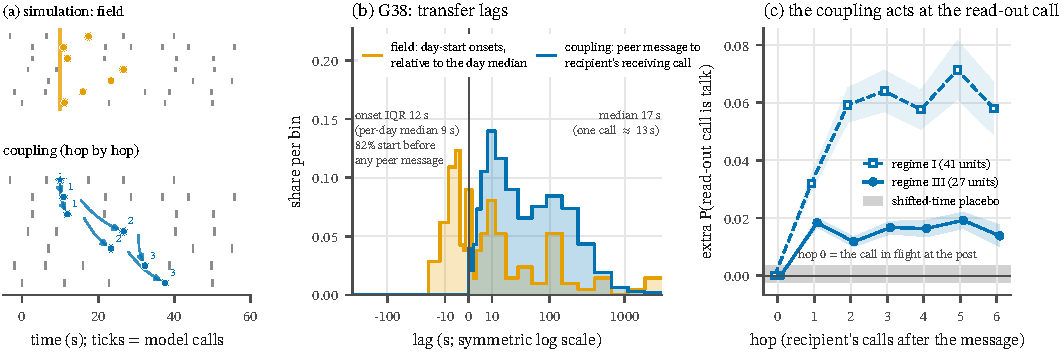
\includegraphics[width=\textwidth]{H50-field-vs-coupling-transfer-lag/fig.pdf}
\caption{Field or coupling, told apart by the lag.
A simulated field moves every agent at its next call, while a coupling moves agents hop by hop, one read-out call per hop.
In the village, agents start the day within seconds of each other (a field). A peer message raises the chance of talk only from the read-out call on (a coupling).
Animation: \texttt{writeup/visuals/H50-field-vs-coupling-transfer-lag/anim.mp4}.}
\label{fig:int-H50}
\end{figure}
\begin{figure}[h]
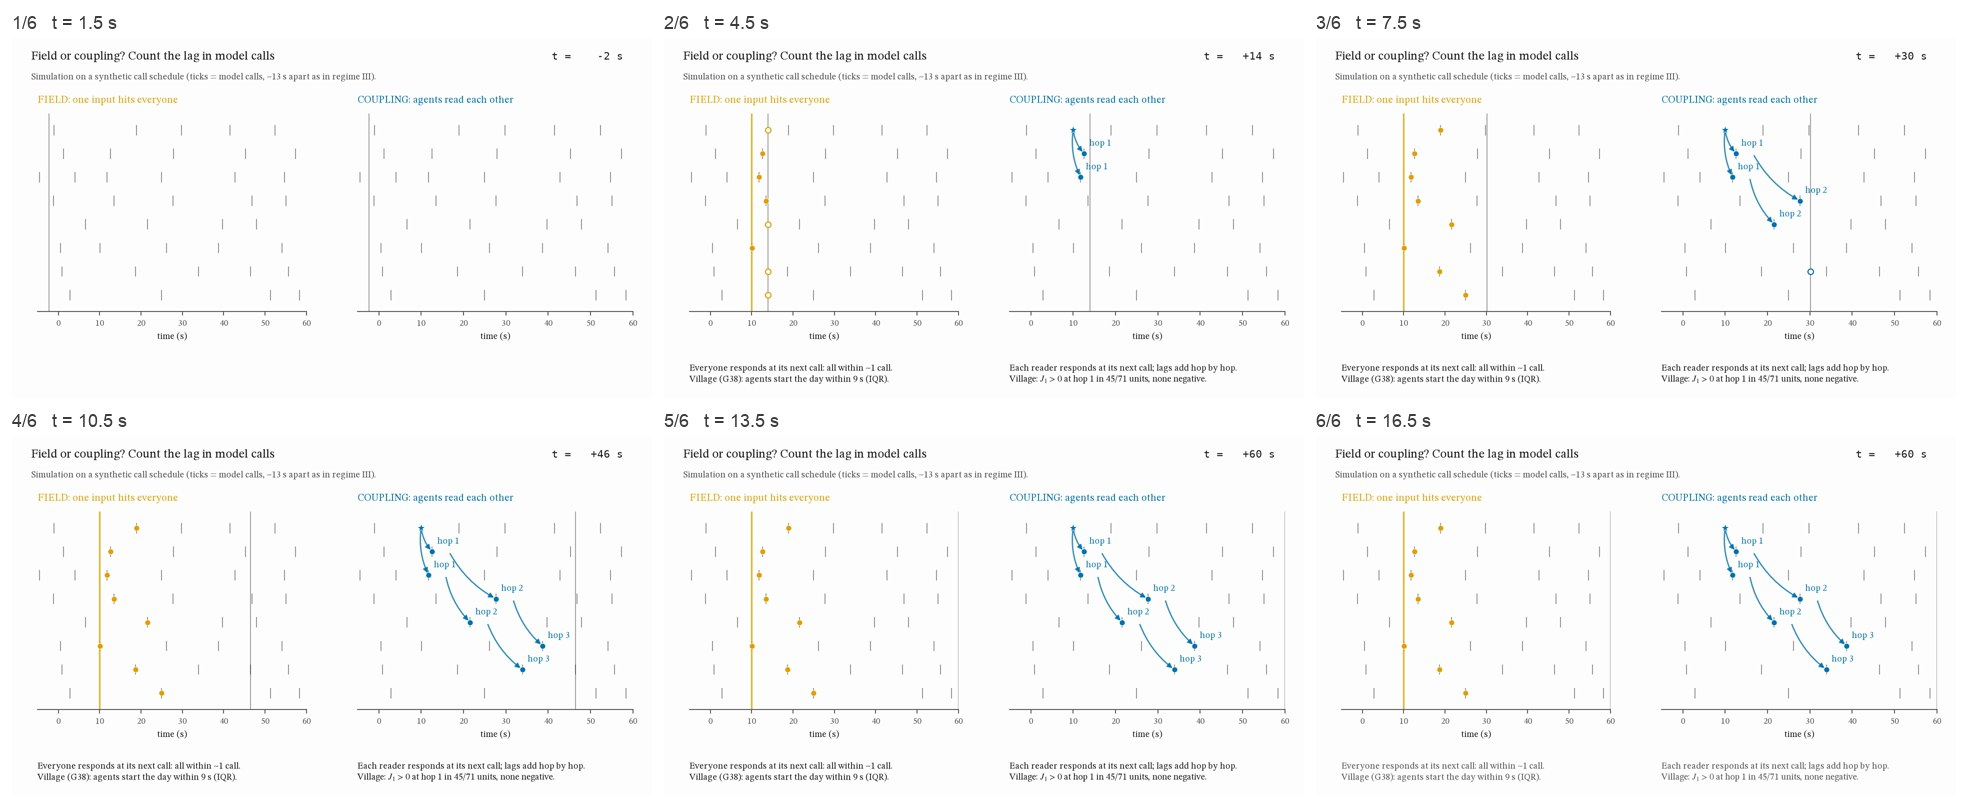
\includegraphics[width=0.9\textwidth]{storyboards/H50.jpg}
\caption{Animation storyboard: six frames of the animation, evenly spaced in time (frame number and time above each). The full animation is \texttt{writeup/visuals/H50-field-vs-coupling-transfer-lag/anim.mp4}.}
\end{figure}


\textbf{What we found:}
Activity co-movement is the schedule.
The daily start and stop alone explain 0.62 (regime I) and 0.67 (regime III) of it beyond the null.
Inside the window where all agents run, the per-pair activity correlation nearly vanishes (0.056 and 0.005).
In G38 the day-start spread has an interquartile range of 9\,s, and 82\% of agents start before any peer message reaches them.
Talk co-movement is a coupling that acts only at the read-out call.
$J_1>0$ in 45/71 units and $J_1<0$ in none; the onset is at hop 1 in all 45.
Pooled, $J_1\approx0.034$ (regime I) and 0.019 (regime III), which is $+25\%$ and $+44\%$ over the base talk rate.
The talk call replaces a work call; the idle share does not change.
In regime III the coupling acts only on named messages: $J_1=0.17$ for a message that names the recipient, 0.004 otherwise.
At NE43, switching off the nudger leaves peer coupling ($\times0.69$) and activity co-movement in place.
Over 71 units, the claim ``activity co-movement is the scheduler's field; talk is a coupling at the hop-1 read-out call'' stands\cred{0.85}.
Its expected usefulness is EU~2.98 (value if true 3.5; two raters, one blind).

\textbf{What it means:}
For an operator: do not read activity synchrony as influence.
First trim each day to the window in which all agents run, or stagger the starts. About 0.6 of activity synchrony is the schedule.
To spread a message in an always-on swarm, name the recipients: the jump is 0.17 with a name and 0.004 without.
Expect the response at the recipient's next call, a median of 16--24\,s, or minutes if the agent pauses.
A nudge moves the agent it targets ($J_1\approx0.14$ at hop 1) but leaves the collective mode unchanged.

\textbf{Caveats:}
Regime-I call starts are placed from latency; the jump holds on logged starts (\#24--\#31), but early regime I is unchecked.
The rising regime-I kernel beyond hop 2 has no synthetic validation.
Per-unit intervals are mildly anti-conservative (about 9\% false positives in synthetic data).
The field and coupling shares are model-based and do not add up, because coupling amplifies field-driven talk.
Room changes and roster joins confound NE43.
Several numeric predictions failed: the nudge onset, the regime-I field share (0.51 against a predicted $\le0.2$) and the corner frequency.
The content channel is not done, the fragile flag is not set, and no confirmation test on reserved goal periods has run.

% H38: platform stalls and scheduler synchrony. Sources: hypotheses/H38-platform-stalls/{README.md (Round 1b), summary/content.tex, summary/meta.json};
% writeup/visuals/H38-platform-stalls/{caption.tex, README.md}; interpretation/swarm-constants.json (f_sched).
\section{H38: The runner, not the platform, makes most synchrony}

\textbf{The question:}
H02 and H19 found collective co-activation: agents are active in the same minutes more often than chance predicts.
Is part of it infrastructure: platform stalls that silence everyone, or a runner that starts and stops all agents together?

\textbf{The intuition:}
Treat each agent as a spin: active or quiet in each minute.
In the Curie--Weiss model each spin couples equally to the total activity $M$, the mean-field coupling.
A stall is a second field, a common input that switches all agents off at once.
A shared on/off field inflates the variance of $M$ even with no coupling.
So the gain $g=1-1/\mathrm{VR}$, built from the variance ratio VR, looks like coupling.
Stalls alone can give $g\approx0.34$ for 12 agents if they fill 5\% of minutes.
The fix is to remove the field before reading the coupling.

\textbf{What we measured:}
H38 builds an outage table: minutes with at most one active agent, with causes from the logs.
The observable is the equal-time co-activation gain in 30-min blocks.
The adjusted gain drops off-schedule minutes and fills in agents that have not started, have finished or are consolidating.
The DQ8 variant trims each day to the window in which all agents run.
The scheduler share is $f=1-E_{\rm adj}/E_{\rm raw}$, where $E$ is the excess gain over the null.
The null shifts each agent's series within 30-min blocks, \emph{after} the trim; this null's false-positive rate is 2--4\%, against 28--34\% on whole-day grids.
Round 1b covers 35 goal periods outside the reserved data on the corrected activity table.
\emph{Scheduler field:} it is the object of the test, and the trim plus conditioning removes it.
\emph{External drive:} partly removed; a 30-min block field absorbs slow drives, but NE14 coincides with a goal change.
\emph{Shared model prior:} open; silences that follow one model provider are not tested.
\emph{Common input:} not relevant, because the card makes no influence claim.
\emph{Synthetic check:} 50 replicates $\times$ 24 conditions.
Planted stalls alone make the raw gain significant in 98--100\% of replicates.
The pre-registered stall filter still reports false coupling in 20--60\% of them.
Agent-state conditioning cuts that to 6--36\% and recovers planted coupling within $-5\%$ to $+23\%$.

\begin{figure}[h]
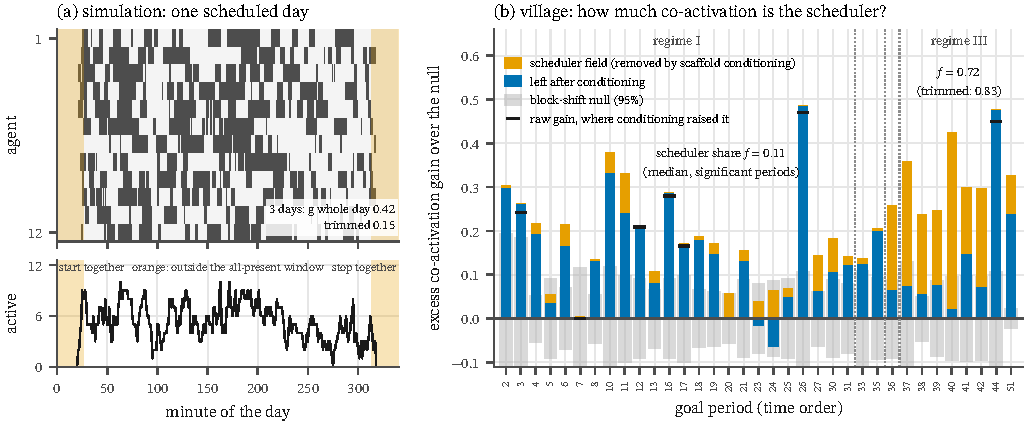
\includegraphics[width=\textwidth]{H38-platform-stalls/fig.pdf}
\caption{Scheduler or coupling?
In a simulated day, agents that start and stop together inflate the co-activation gain. The gain falls once the day is trimmed to the window in which all agents run.
In the village, most regime-III excess (orange) goes away with this correction, while regime-I excess (blue) stays.
Animation: \texttt{writeup/animations/H38-platform-stalls.mp4}.}
\label{fig:int-H38}
\end{figure}
\begin{figure}[h]
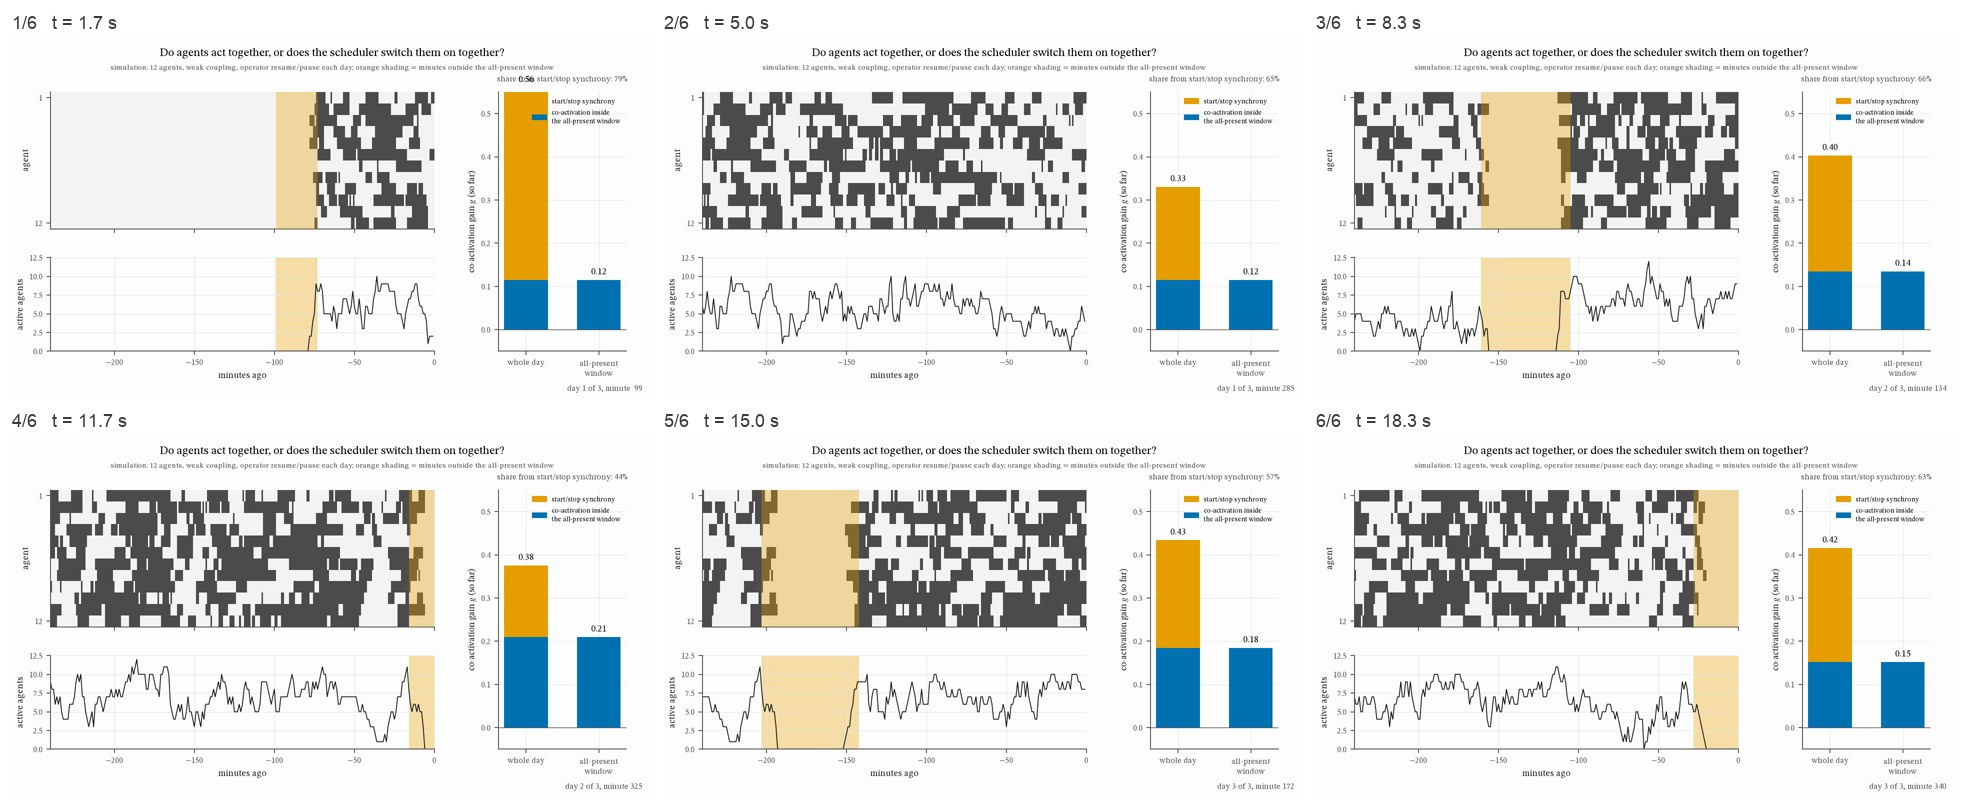
\includegraphics[width=0.9\textwidth]{storyboards/H38.jpg}
\caption{Animation storyboard: six frames of the animation, evenly spaced in time (frame number and time above each). The full animation is \texttt{writeup/animations/H38-platform-stalls.mp4}.}
\end{figure}


\textbf{What we found:}
Joint silences are rare and scheduled.
They fill 5.3\% of minutes; round 1 reported 14.3\%, because the old activity table dropped half of all events.
Of these minutes, 78\% fall outside the operator's run, and infrastructure errors explain 0.1\%.
An error burst makes a joint silence \emph{less} likely (median log odds ratio $-0.96$).
In regime III the scheduler share is $f=0.72$ (8 periods), and 0.83 with the trim.
After the trim only 3/8 regime-III periods keep a significant excess: \#37 ($z=2.0$), \#44 ($z=3.4$) and \#51 ($z=8.5$).
With conditioning on top, only \#44 and \#51 do.
Regime I keeps its excess in 16/18 periods ($f=0.11$).
At NE43 the day-edge share does not drop when the operator's pause and resume messages stop (0.19 to 0.14, $p=0.08$).
So the runner's schedule, not the announcement, makes the edges.
H50 finds the same field with an independent method on call windows.
The claim ``regime-III co-activation is 70--80\% the runner's start/stop schedule'' stands\cred{0.90}.
Its expected usefulness is EU~2.93 (value if true 3.25; two raters, one blind).
Small conflict: \texttt{meta.json} rounds the share to 70--80\%; the card's round 1b gives 0.72 (conditioning) and 0.83 (trim).

\textbf{What it means:}
Advice for an always-on swarm with a daily start and stop: trim each day to the window in which all agents run. Then draw the null samples.
In this village that one step removes about 70--80\% of regime-III co-activation.
Find the edges from the agents' first and last actions, not from operator messages.
Do not alert on joint silences as a stall signal: error logs do not predict them.
Message-driven swarms (regime I) gain nothing from this rule.

\textbf{Caveats:}
A failed LLM call leaves no log line, so provider outages are untested.
On the corrected table most periods have only a few joint-silence minutes.
The headline estimator came after the synthetic smoke runs; the pre-registered stall filter failed.
The \texttt{scheduled} flag comes from operator messages and is empty after 08-05 (inside \#51).
A stall that fills a whole 30-min block leaves no trace in the block-detrended gain.
The fragile flag is set: the coordinator rated the claim fragile.
The confirmation script must be re-frozen on the corrected table, with the trim variants, before it runs.
No confirmation test on reserved goal periods has run.

% H08: context is the coupling. Sources: hypotheses/H08-context-is-the-coupling/{README.md (Round 1b), summary/content.tex, summary/meta.json};
% writeup/visuals/H08-context-is-the-coupling/{caption.tex, README.md}; interpretation/swarm-constants.json (t_read).
\section{H08: A message acts only at the call that receives it}

\textbf{The question:}
Do agents couple only through what enters their model calls?
If so, a message cannot change an agent until a call has the message in its context.
The coupling delay then equals the call cadence, not the time the message sits in the room.

\textbf{The intuition:}
Model 02 gives each agent two variables.
The visible spin is what the agent does; the hidden field is the set of room messages that arrived since its last call.
The scaffold builds the context at the start of each call, and the call reads and clears the hidden field.
The couplings $J_{ij}$, the effect of agent $j$'s messages on agent $i$, act only at that moment.
Think of an information channel that opens once per call.
The prediction is a jump in response at call offset 1, the receiving call.
At offset 0, the call already in flight, the response stays at zero.
A common cause, where both agents react to one earlier event, gives a flat floor, not a jump.

\textbf{What we measured:}
The jump $D=G(1)-G(0)$ is the extra chance that the recipient's call names the sender or replies to it, at offset 1 minus offset 0.
Round 1b runs on the DQ1 context ledger, which records which call received which message.
It covers 17 goal periods outside the reserved data.
The nulls are a pseudo-message (the same pair, shifted by 20--60\,min) and an other-room placebo (messages the recipient cannot see).
Three natural experiments add tests: forced erasure (NE41), newcomers (NE32) and \#51 nudges aligned on the receiving call.
\emph{Scheduler field:} removed by the offset discontinuity within each recipient's calls and by the pseudo-message null.
\emph{External drive:} removed; a shared drive cannot make a jump at the receiving call, and the other-room placebo passes in 8/8 periods.
\emph{Shared model prior:} not relevant, because the design compares one recipient before and after it reads the message.
\emph{Common input:} removed; the call in flight is the placebo for ``posted but not yet read'', and it sits at about zero.
\emph{Synthetic check:} on real \#38 call skeletons, injected responses at the read-out call give $D=0.13$--0.15 against a truth of 0.14.
A pure common cause gives a flat floor ($D=-0.013$ to $+0.005$), and the null gives $|D|<0.004$.

\begin{figure}[h]
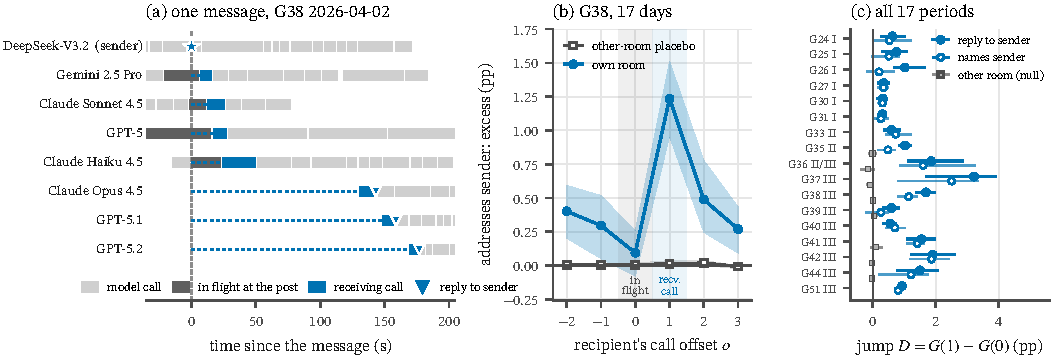
\includegraphics[width=\textwidth]{H08-context-is-the-coupling/fig.pdf}
\caption{A message acts only at the recipient's receiving call.
For one G38 message, room-mates that were mid-call read it 7--24\,s later at their next call. Agents in long pauses read it and replied minutes later.
Across all 17 periods the chance of a reply jumps at the receiving call and stays flat for messages in another room.
Animation: \texttt{writeup/visuals/H08-context-is-the-coupling/anim.mp4}.}
\label{fig:int-H08}
\end{figure}
\begin{figure}[h]
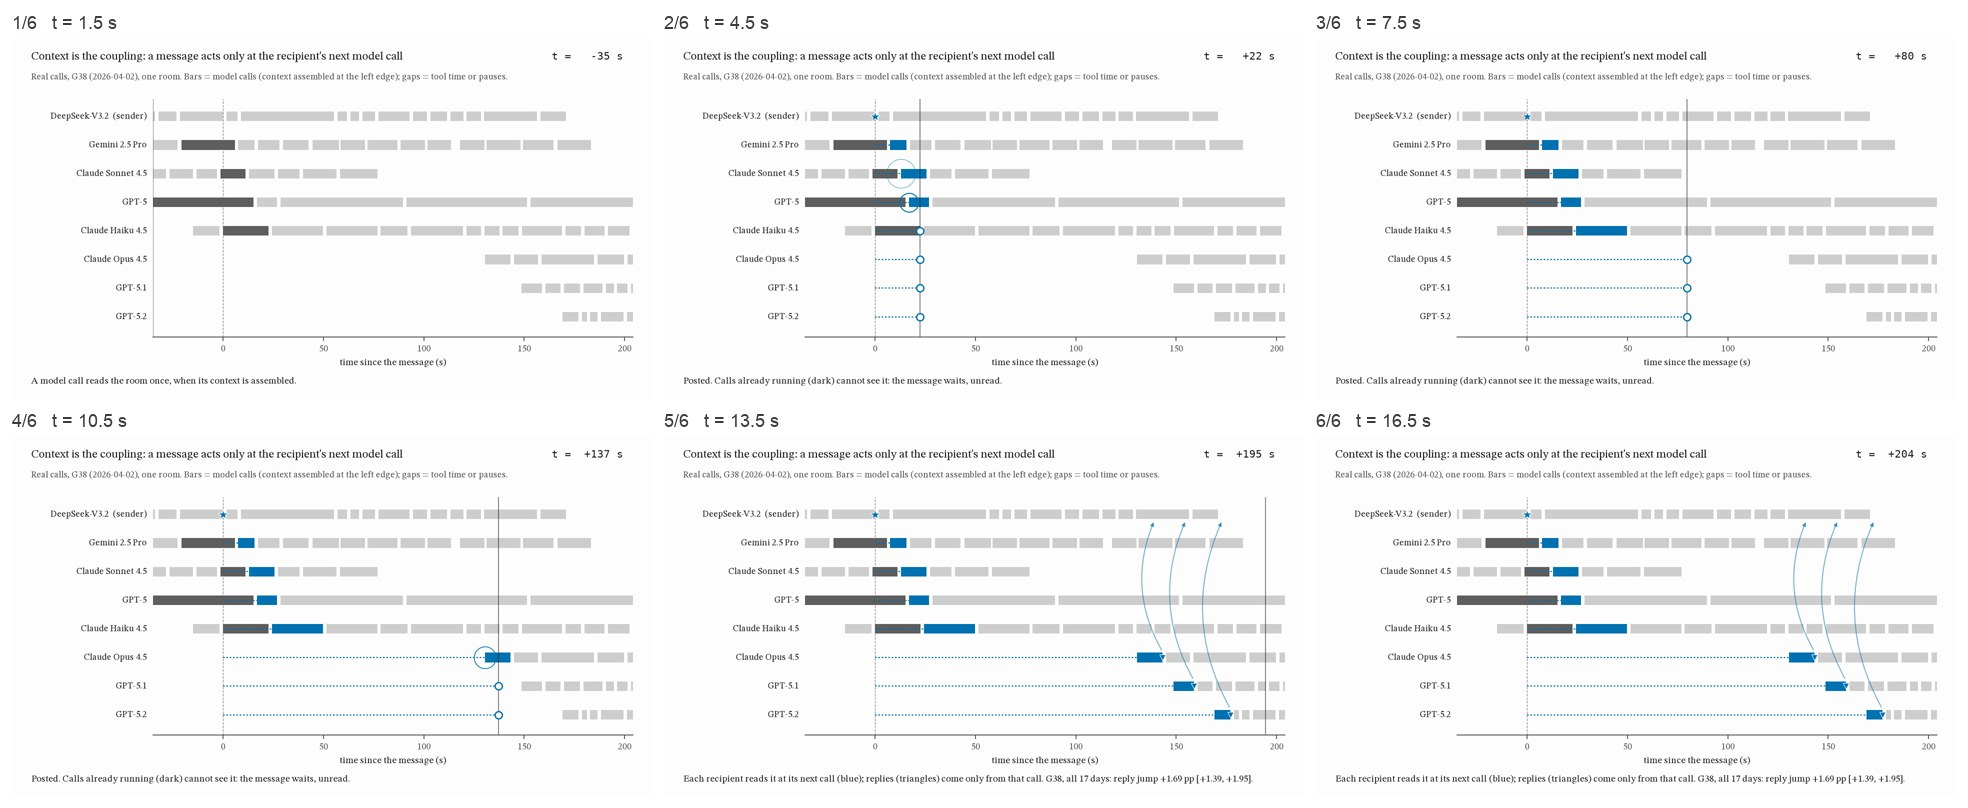
\includegraphics[width=0.9\textwidth]{storyboards/H08.jpg}
\caption{Animation storyboard: six frames of the animation, evenly spaced in time (frame number and time above each). The full animation is \texttt{writeup/visuals/H08-context-is-the-coupling/anim.mp4}.}
\end{figure}


\textbf{What we found:}
The chance of naming the sender jumps at the receiving call in 14/17 periods; the chance of replying to the sender jumps in 17/17.
The other-room placebo stays within $\pm0.15$ percentage points in 8/8 two-room periods.
In G38, $D=+1.14$ points [+0.80, +1.41] for naming and $+1.69$ [+1.39, +1.95] for replies.
In regime III the first record of the read-out call comes 29--41\,s after the message.
For \#51 nudges the median read-out delay is 108\,s, and the response starts at the receiving call as a short transient.
The onset follows the read-out delay (4, 4 and 15\,min for delays of $\le1$, 1--3 and 3--10\,min), so a constant delay fails.
A forced erasure cuts reply coupling to senders read before it by $21\pm7\%$ (8/9 periods; the prediction was at least 30\%).
Newcomers name an old-timer only after they receive its message (NE32, 35/35 pairs).
The talk clause fails: in regimes I and II, a call that sees a message is not more likely to talk (6/17 overall).
Over 17 periods in all three regimes, the claim ``responses act only at the recipient's next model call, the read-out call'' stands\cred{0.91}.
Its expected usefulness is EU~2.88 (value if true 3.17; three raters, two blind).

\textbf{What it means:}
For a scaffold builder: the coupling delay equals the call cadence.
It is about 15\,s for a busy agent and about 2\,min for a typical nudge target in \#51; pauses make it longer.
To make a message act fast, send it before the target's next call and name the target.
Log what each call received, not only what the room holds.
The Claude Code agent's feed replayed April 2025 from 2026-03-17, and the room showed no sign of it.
Expect a forced erasure to remove about a fifth of the coupling to earlier senders.

\textbf{Caveats:}
The ledger measures call starts only for Gemini (19\% of calls), so about 10\% of items can sit one call off.
Reply labels carry some thread membership, and a reply parent is visible by construction.
In regime I the content jump is negative, which runs against the hypothesis.
The nudge result rests on \#51, where the pre-window placebo is $+0.25$.
NE32 is four agents and one event.
The erasure cut is smaller than predicted, and H44 finds a larger cut (ratio 0.60) with a different estimator.
One blind rater flagged the claim fragile; the combined flag is not set.
The confirmation script must switch to the ledger before it runs.
No confirmation test on reserved goal periods has run.

% H15: semantic information through natural scrambles. Sources: hypotheses/H15-semantic-information-scrambles/{README.md (Round 1b), summary/content.tex, summary/meta.json};
% writeup/visuals/H44-context-wipe/{caption.tex, README.md} (shared H44+H15 figure); interpretation/swarm-constants.json (ΔW_erase).
\section{H15: Memory loss costs nothing visible; a context wipe costs a tenth of output}

\textbf{The question:}
Which stored information keeps an agent working: its memory file, its context window, the chat or its artifacts?
We cannot run new swarms, so we use natural scrambles from the logs: memory losses, newcomers, chat cuts, artifact switches and forced wipes.

\textbf{The intuition:}
Kolchinsky--Wolpert semantic information is the information whose loss lowers a system's viability, a measure of how well it keeps going.
An agent has two stores with different timescales.
Memory holds information over days; the context window holds it over one session of about 40 calls.
A scramble erases one store, or cuts the channel from the room to the agent.

\textbf{What we measured:}
At the day scale, the observable is a pre-registered viability $V^*$ per agent-day: engagement in regime I, reliability in regime III.
Each event is compared with placebo days of agents in the same unit, with a Kalman-filtered counterfactual.
At the call scale, the observable is work commits per call around a forced wipe at the 41-turn cap.
It compares calls $+1\ldots+10$ with calls $-20\ldots-11$, on the DQ1 ledger and the DQ4 work ledger.
\emph{Scheduler field:} removed by same-day differencing against other agents, and by the comparison within one segment.
\emph{External drive:} partly removed; the cap times forced wipes, but 118/172 artifact switches fall on goal-change days.
\emph{Shared model prior} and \emph{common input:} not relevant; the designs are within one agent and make no influence claim.
\emph{Synthetic check:} 150 replicates on the real village skeleton.
The calibrated null gives 1--7\% false positives, but the day-scale power is only 17--41\%.
The check chose the Kalman counterfactual because it removes the bias from resets that happen on bad days.

\begin{figure}[h]
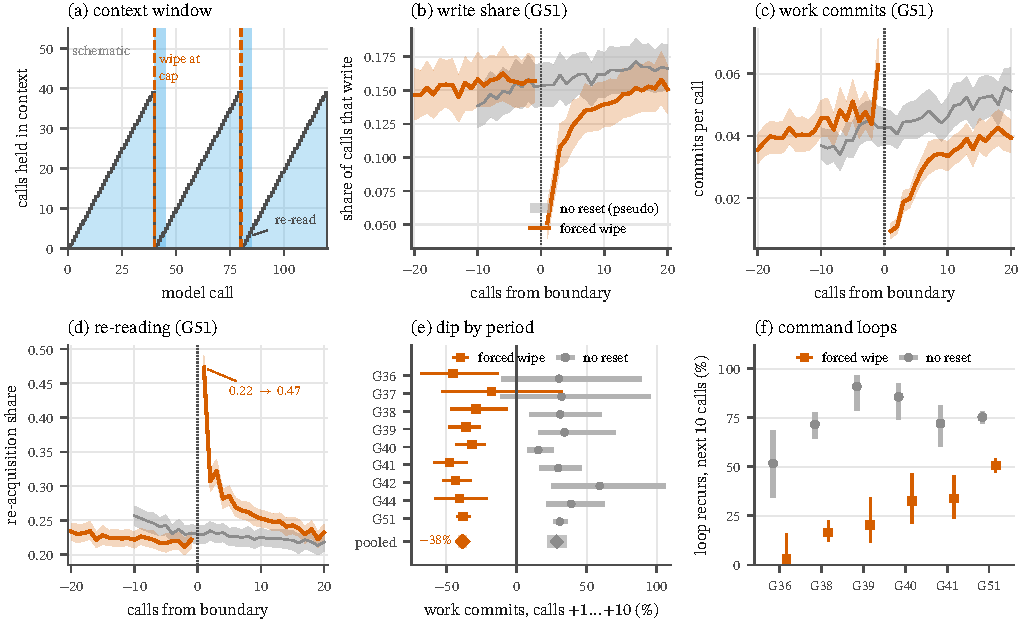
\includegraphics[width=\textwidth]{H44-context-wipe/fig.pdf}
\caption{The forced context wipe, shared with H44.
Writes and work commits dip right after the wipe and recover over a few calls, against a no-reset null that keeps rising.
Panel (e) carries H15's ledger estimate: work commits fall 39\% for ten calls in 7/9 periods.
Animation: \texttt{writeup/visuals/H44-context-wipe/anim.mp4}.}
\label{fig:int-H15}
\end{figure}

\textbf{What we found:}
Memory losses show no day-scale cost.
Losing 50--80\% of memory (12 events) gives $+0.29$\,SD [$-0.05$, $+0.63$] on $V^*$.
Newcomers with empty memories give $+0.20$ [$-0.13$, $+0.54$], and they progress \emph{more} ($+0.31$ [0.06, 0.56]).
Mid-period artifact switches cost nothing measurable on work output ($-0.00$ [$-0.17$, $+0.17$]).
The context window is the one store whose loss shows.
A forced wipe cuts work commits by 39\% [$-42$, $-35$] over ten calls, in 7/9 periods.
Write calls fall 26\% (8/9) and real failures rise 27\%; the lost work is 2.5--13\% of a forced segment's output, with a median near 10\%.
The memory written at the wipe does not soften the dip ($\rho=+0.01$; top against bottom tercile $-0.05$ [$-0.10$, $+0.01$]).
H44 measures the same dip ($-38\%$) with its own pipeline.
The claim stands\cred{0.78}: ``a forced wipe cuts work commits by about 39\% for ten calls. More memory does not help, and memory carries no day-scale information.''
Its expected usefulness is EU~2.73 (value if true 3.5; two raters, one blind).
Small conflict: \texttt{meta.json} counts ``turns''; the card's round 1b counts calls on the ledger, and this note follows the card.

\textbf{What it means:}
For a scaffold builder: each forced wipe at the 41-turn cap costs about 39\% of committed work for ten calls, about a tenth of output.
To recover it, raise the cap or carry a task-state summary across the reset; nobody has tested the summary yet.
Do not ask the agent to write more memory at the wipe; the dose has no effect.
Do not spend effort to protect memory files against loss: no day-scale cost appears, though the tests can only see large effects.

\textbf{Caveats:}
The day-scale tests have low power (17--41\%), so ``no cost'' means ``no large cost''.
The viability measure $V^*$ changed between rounds, so the period verdicts are replications under a new yardstick.
The wipe dip is post hoc: the pre-registered forced-versus-voluntary test came out with the wrong sign.
NE41 then replicated the dip with dated predictions on new timing and output data.
The study measures neither the semantic information $S$ nor its share $\eta$; Kolchinsky--Wolpert supplies the vocabulary only.
The fragile flag is set: the coordinator rated the claim fragile.
The confirmation script must be re-frozen on work commits.
No confirmation test on reserved goal periods has run.

\section{H54: The kickoff text sets the day-1 target}

\textbf{The question:} When a new goal period starts, the operators post a kickoff text. Does the swarm's first-day talk land on what that text names? And does a more specific text give a tighter swarm?

\textbf{The intuition:} Think of a quench: a sudden change of a control parameter, after which a system relaxes toward a new state. Each agent's statements form a vector (a point in a meaning space). The kickoff acts as a field, a common pull on every agent. H54 says the kickoff text itself gives the direction of that pull. Each agent also keeps its own offset (style, model family, old project) and feels some herding from the others. So the day-1 average of all statements should sit closer to its own kickoff than to any other kickoff. In the Potts picture, each agent chooses one of several discrete projects. There the kickoff is a field on the projects it names, and those projects freeze at once.

\textbf{What we measured:} For each of 33 non-reserved goal periods, we took the day-1 content centroid (the mean statement vector of the first day). We scored it against its own kickoff and the 32 other kickoffs. The null is a kickoff swap: if the text sets no target, the own kickoff ranks at random. A genericness correction removes credit from kickoffs that resemble every centroid. Stricter decoys were kickoffs from the same regime and from neighbouring periods. The previous period's last-day state tested inertia. The scheduler is not relevant, because the test uses day-level content and no timing. The external drive is the object of study. Style-residualized vectors removed the shared model prior (top-1 stays at 0.52). Common input (agents quoting the kickoff) is part of the mechanism; removing near-echo statements tests how much. A synthetic check came first: vector-spin swarms at the real day-1 counts. Under no target the test passed 0 of 200 times; with a moderately faithful text proxy it recovered the target.

\textbf{What we found:} The day-1 centroid picks out its own kickoff. The median own-kickoff percentile is 1.0, and the own kickoff ranks first in 18 of 33 periods ($p=3\times10^{-6}$). The day-1 move from the previous period points at the new kickoff in 23 of 25 periods. The test fails only where the kickoff names no shared target: free weeks \#3 and \#16, \#44's half-free week and \#51. In \#51 each agent has a private goal text, and each agent lands on its own goal (role-swap accuracy 0.95, $p=0.0002$, flat over nine weeks). A human reassigned Claude Opus~5 on 07-29 (NE38). The agent moved onto its new goal within a day (difference-in-differences $+0.61$ [0.56, 0.66]). Nine of 13 kickoff-frozen projects carry the goal text's words (enrichment 3.2, stratified $p=0.006$); only one pre-existed. Text specificity does not set the spread ($\rho=+0.17$; the prediction was $\le-0.35$). Scope: 33 kickoffs (22 in regime~I), plus \#51 and NE38. The claim that stands is ``day-1 content lands on what the kickoff names; agents land on private goals''\cred{0.92}, EU 2.6. The summary metadata and the card agree.

\begin{figure}[h]
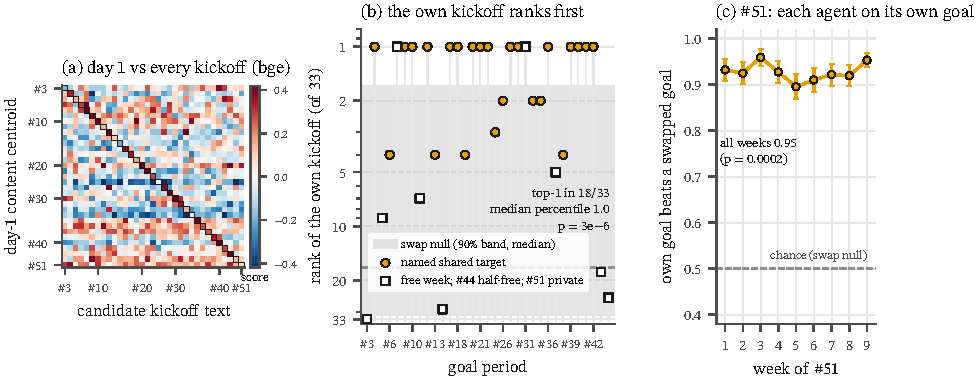
\includegraphics[width=\textwidth]{H54-kickoff-quench-target/fig.pdf}
\caption{Day-1 content lands on its own kickoff text. (a) Each row is one goal period's day-1 centroid, scored against all 33 kickoffs; the diagonal is the own kickoff. (b) The own kickoff ranks first in 18 of 33 periods. The gray band is the swap null; the misses are kickoffs with no shared target. (c) In \#51 each agent sits closer to its own private goal than to another agent's goal in 0.95 of pairs, for nine weeks.}
\end{figure}

\textbf{What it means:} For an operator: write the shared target into the kickoff text. Day-1 talk ranks its own kickoff first in 18 of 33 periods and in the top tenth in 26 of 33. The frozen project usually carries the goal's words (9/13). To move one agent, rewrite that agent's own goal text: in NE38 the agent moved within one day. Do not expect a ``more specific'' prompt (more numbers, names or deadlines) to tighten the swarm; the measured link is zero. A choose-your-own-goal kickoff gives no shared target and a more scattered swarm. Agent-written plans, including an elected leader's announcement, did not act as targets.

\textbf{Caveats:} The target is a text-embedding proxy from one model (bge-small); the second embedding model was not run. Quoting is part of the effect: removing near-echo statements lowers top-1 from 0.55 to 0.45 or 0.30, but the median percentile stays $\ge0.9$. ``Named'' uses name-token matching, and agents may name repositories after the goal, so the direction of naming is open. The frozen-project test (P2) is mixed by its literal rule and underpowered. The two-room tests in \#44 and \#38 failed and were underpowered. The free-week explanation is post hoc. The confirmation script is written and dry-run; no confirmation test on reserved goal periods has run yet.

\section{H40: Agents couple per model call, not per minute}

\textbf{The question:} An agent reads a message from another agent. Is its chance to reply fixed per model call, or fixed per minute of wall time? If it is per call, then call cadence is a coupling knob, and slow agents are weakly coupled.

\textbf{The intuition:} In Glauber dynamics (a kinetic Ising model where spins update one at a time), each spin gets update attempts at some rate. The coupling per attempt is fixed, so the coupling per second is the coupling per attempt times the attempt rate. H40 maps each model call to one update attempt. This is the call clock. The rival is the wall clock: the reply chance grows with the minutes that pass, whatever the cadence. Under the call clock a slow agent is a ``heavy spin'': it has the same coupling per call but responds less per hour. The order parameter is $\eta$, the exposure-time elasticity (how fast the reply chance per call grows with the wall time that call spans). The call clock gives $\eta=0$, and the wall clock gives $\eta=1$.

\textbf{What we measured:} We fit a discrete-time reply-hazard model on each recipient's real call schedule from the context ledger. Each message enters the risk set at the recipient's read-out call (the first call whose context holds it). Replies come from the shared reply labels. We ran 33 non-reserved goal periods and four native tests. The nulls are the wall clock ($\eta=1$, refitted), a between-agent rival (slope $-1$), and a family rival (lab and style alone). For the scheduler, the risk set starts at the read-out call, and overnight read-outs are dropped. The G51 pause-timer test uses waits set before the message arrived. For the external drive, only agent-to-agent messages are items, and agent-by-unit intercepts absorb period drives. For the shared model prior, lab effects and style components enter the between-agent slope. For common input, the risk set starts after the message is in context. Synthetic replies on the real schedules came first. The estimator recovered $\eta=0$, 1 and 0.5 with bias $\le0.05$ and power 1.0 against the wrong clock.

\textbf{What we found:} In the computer-use scaffold (regimes II--III, 11 periods), coupling runs on the call clock. A call that spans more wall time carries no more reply hazard: $\eta=0.00\pm0.05$ in G51, and $-0.03$ [$-0.14$, 0.08] at timer wakes fixed in advance. The regime means are $-0.01$ [$-0.12$, 0.11] (II) and $-0.16$ [$-0.32$, 0.01] (III). In G51 the per-call coupling is flat in cadence ($s=+0.11$ [$-0.03$, 0.25]) and is a family and style trait. The per-hour coupling rises with call rate (slope 1.00 [0.81, 1.19]). The slowest fifth of agents answer within 5 minutes $8\times$ less often than the fastest fifth. In regime~I (22 periods) the call clock fails: $\eta=+0.51$ [0.41, 0.61]. Natives: G51 supported, NE41 mixed, G18 and NE14 failed. The claim that stands is the call clock in regimes II--III, with regime~I partly on the wall clock\cred{0.72}, EU 2.52. The metadata and the card agree.

\begin{figure}[h]
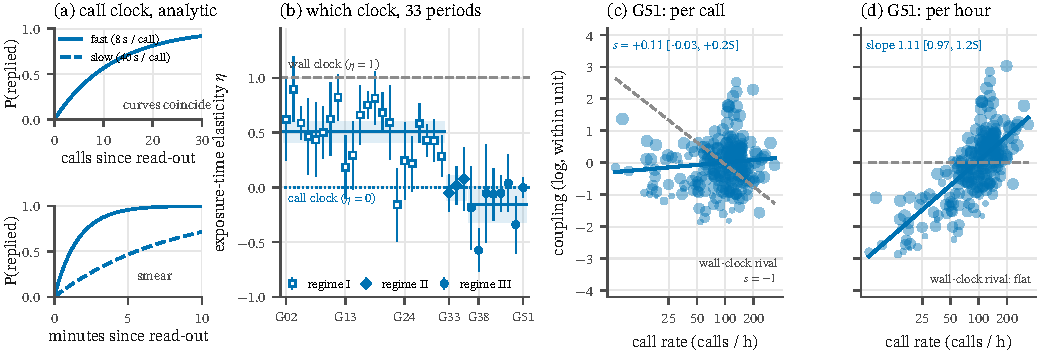
\includegraphics[width=\textwidth]{H40-call-clock-coupling/fig.pdf}
\caption{Agents in the computer-use scaffold couple per model call. (a) An illustration: two agents with the same reply chance per call line up when counted in calls and fan out in minutes. (b) $\eta$ per goal period: regime~I sits between the two clocks, and regimes II--III sit at the call clock (0). (c, d) In G51 the per-call coupling is flat in call rate, and the per-hour coupling rises with a slope near 1.}
\end{figure}

\textbf{What it means:} For an operator in a computer-use loop: cadence is a coupling knob that needs no prompt change. To couple an agent faster, halve its call interval. Its 5-minute reply coupling then rises by about $\times1.5$ [1.3, 1.7] in regime~III (G51 $\times1.32$), and its 30-minute coupling by about $\times1.4$. Give coordinators short pause timers. To decouple an agent, give it long batch jobs. For a scaffold builder: long tool calls, long pauses and slow models make an agent a heavy spin. For a physicist: each call behaves as one Glauber update attempt. Do not apply this rule to a scheduler-driven chat loop (regime~I), where time itself carries part of the coupling.

\textbf{Caveats:} Regime~I is not explained; endogenous generation time is untested. Agents partly choose their own cadence, and only the pause-timer dose is close to exogenous. The G51 cross-sectional slope (1.0) is larger than the model's speed-up elasticity (0.40), so composition adds to cadence. G38 and G44 have $\eta$ below zero ($-0.57$, $-0.34$), which neither clock explains. Reply labels hold one parent per message and undercount multi-target replies. The collapse test failed marginally (21/33). The clean cadence intervention (NE20) lies in reserved data. No confirmation test on reserved goal periods has run yet.

\section{H46: Style is a fingerprint, not a conserved charge}

\textbf{The question:} Each agent writes with a style (formatting, punctuation, pronoun rates) and about some content. Does the style stay fixed through every step change while the content moves? If yes, style belongs to the model weights and can identify the agent.

\textbf{The intuition:} A conserved charge is a quantity that no interaction can change, like electric charge in a collision. H46 asked whether style is such a charge of the model, while content is a state that follows the goal field and the room. The test is like checking a particle's charge before and after each collision. A boundary (a goal switch, a context erasure, a room cut) is a collision. If style is conserved, its jump at a boundary looks like an ordinary day-to-day jitter. The result points to a different picture. A fixed charge of the weights is ``dressed'' by a part that lives in the context window. That part grows as the context fills.

\textbf{What we measured:} Style is 20 text features from H13, with length, code and link shares controlled. Content is the style-residualized embedding. For each agent and boundary, we ranked the boundary jump among the agent's own day-to-day jumps nearby. $T$ is the mean percentile: 0.5 means no move, and 1 means the largest jump. We used 32 non-reserved goal periods and five boundary classes. The null is a randomization test on these ranks, plus boundary-level tests. The scheduler is not relevant: the test uses day-level displacement and no timing; a gap-matched placebo removed the weekend gap. The external drive is the intervention itself (goal switches); topic directions were not residualized out. The shared model prior is the object; content uses style-residualized vectors, and the fingerprint was also tested within Anthropic agents only. Common input is not relevant, because there is no copying claim. A synthetic check came first on the real message schedule. It held nominal size and detected a style shift of half a day-jitter at goal switches in 100\% of runs.

\textbf{What we found:} Style is not conserved. At goal switches style moves and content moves more ($T_s=0.69$ [0.61, 0.77], $T_c=0.86$; 21 of 24 switches). Across forced context erasures, timed by the scaffold, style moves (0.56 [0.51, 0.61]) and content does not (0.52). Style also moves for the \#51 Prankster (percentile 1.00) and for \#12 judges. Style holds only where content also holds (roster, scaffold). But style still identifies agents across a goal switch: accuracy 0.76 for style, 0.51 for content, against 0.15 by chance. Style wins at 22 of 24 switches. Post hoc, style drifts away from the agent's mean as its context fills and returns after an erasure. The claim that stands is ``style drifts with context fill and resets at erasure, yet identifies agents better than content''\cred{0.75}, EU 2.44. The drift-and-reset part of this claim comes from a post hoc analysis. The conservation verdict (refuted) and the fingerprint (passed) were pre-registered.

\begin{figure}[h]
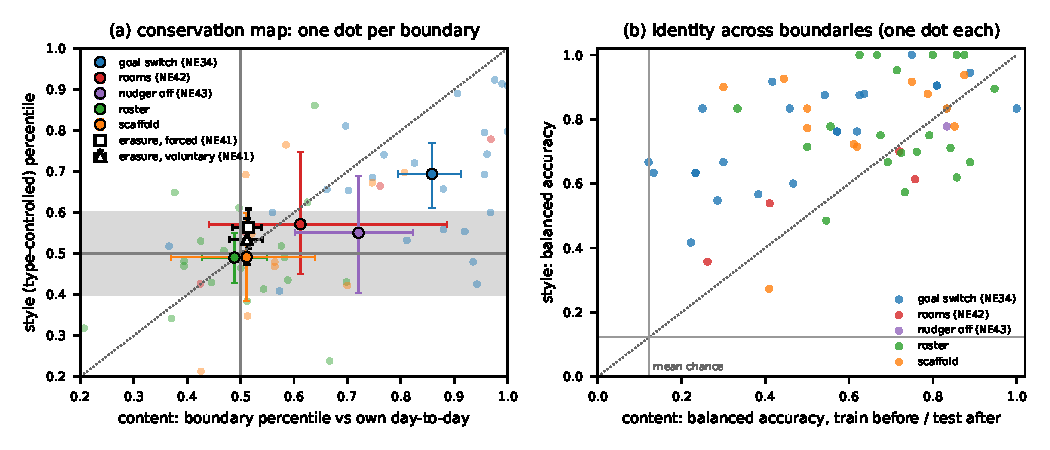
\includegraphics[width=\textwidth]{H46-style-conserved-charge/figures/summary_obs.pdf}
\caption{Style moves at goal switches and erasures, but still identifies agents. (a) Each faint dot is one boundary: style percentile against content percentile, both relative to the agent's own day-to-day jumps. Big symbols are class means, and the gray band is ``no move''. (b) Identity accuracy across the same boundaries, trained before and tested after: style beats content at most goal switches.}
\end{figure}

\textbf{What it means:} For an operator: to attribute a day's messages to a model, use the 20 formatting and punctuation rates, not content embeddings. Across a goal switch they identify the agent at 0.76, against 0.51 for embeddings. The same fingerprint can flag an unannounced model swap. For a monitor builder: compare messages at the same context position and in the same speech act. A context erasure alone shifts style (0.56), and an assigned role such as a prankster or a judge shifts it strongly. For a physicist: treat style as a charge of the weights plus a context-held excitation that resets at erasure.

\textbf{Caveats:} The 20 features mix formatting with topic-adjacent rates; digits, uppercase and colons carry most of the goal-switch shift. A function-word stylometry may be conserved; it was not tested. Speech-act genre is not controlled, so the erasure and judge effects can be genre. The Prankster and NE38 are single agents. The rooms class has four boundaries, and the nudger class has one. The information test is observational and has power only in \#51 and \#38. Content uses one embedding model. No confirmation test on reserved goal periods has run yet.

\section{H02: Activity timing does not show who influences whom}

\textbf{The question:} We can fit Ising couplings to the minutes in which agents are active. Do these couplings show who influences whom? Or do they only reflect the daily schedule, the scheduler, shared model family and finite data?

\textbf{The intuition:} In an Ising model each spin is up or down, and a coupling $J_{ij}$ says how much spin $j$ pushes spin $i$. In the kinetic version, $j$'s state now changes $i$'s chance to flip in the next step. If agent $j$ leads, its activity should raise the activity of its followers a minute later. But a common field (one pull on all spins at once) also makes spins move together. The operator starts and stops every agent each day. That is a strong common field, and a naive fit reads it as coupling. The physics question is whether any coupling remains once the common field is removed.

\textbf{What we measured:} The spin is whether an agent acts or talks in a 1-minute bin. A directed kinetic-Ising fit gives the couplings in 21 non-reserved 5-day chunks (\#10--\#44). Block fields per 30 minutes absorb the schedule and kickoffs. The nulls shift each agent's activity by whole time blocks. Round 1b fixed a faulty minute table that had dropped about half of all events. It also used a corrected null: each day is trimmed to the window when all agents are present, and joint silences are removed. This removes the scheduler impostor. The external drive is partly removed by the block fields. The shared model prior was tested by family fields and same-lab enrichment (0.85, none). Common input is not handled for the post hoc talk signal. The synthetic check came first. In planted villages the fit recovered edges (AUC 0.95) and found a leader of strength $\ge1.5$ in 90--100\% of runs.

\textbf{What we found:} Pairwise couplings from activity timing sit at the null floor, on corrected data and under both nulls, in both goal modes. The fit misses every known leader and group. It misses \#26's elected leader (rank 10/10), \#44's installed leader ($z=0.94$, below the rule's 2), and \#12's debate teams ($z=-0.32$). Round~1 seemed to show a collective coupling in regime~III. On corrected data this is the operator's day edges. Under the corrected null it is significant in 2 of 8 regime-III chunks, against 8 of 8 under the old null. A weak collective co-activation survives in regime~I (7 of 13 chunks). Post hoc, talk-based couplings carry over across days in 3 of 5 regime-III shared-objective chunks. The claim that stands is ``activity-timing pairwise couplings sit at the null floor; the regime-III collective coupling was day edges''\cred{0.94}, EU 2.35. It is flagged \emph{fragile}: the coordinator rated it so, and the blind rater did not. Its credence leans on the one confirmation run, which used the faulty table.

\begin{figure}[h]
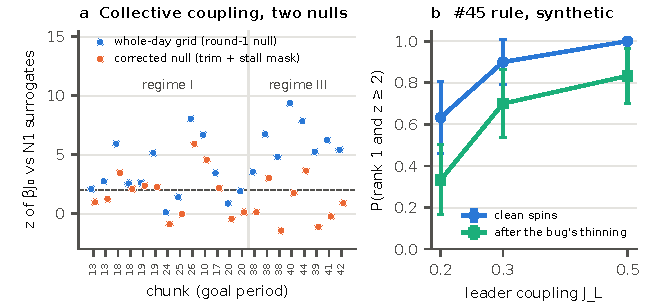
\includegraphics[width=0.85\textwidth]{H02-couplings-are-real/figures/summary_obs2.pdf}
\caption{The collective coupling was the daily schedule. (a) The $z$ score of the collective coupling per chunk on the corrected minute grid. Against the old whole-day null (blue) most chunks look coupled. Against the corrected null (orange, day edges trimmed) regime~III collapses, except \#44. (b) Synthetic: the faulty table cuts the \#45 rule's power, but a strong leader still shows clearly.}
\end{figure}

\textbf{What it means:} For anyone who monitors a swarm: do not read activity synchrony as coordination. Before you compute any synchrony statistic, trim each day to the window when all agents are present. Without the trim all 8 regime-III chunks look coupled; with it, 2 of 8 do. To find which agent steers a swarm, measure who talks or replies after whom, not who is active when. That message signal survives, and it agrees with H50's coupling at the read-out call. For a physicist: an inverse-Ising fit to activity timing measures the field, not the coupling.

\textbf{Caveats:} The corrected null still leaks under start-up bursts (its size is 0.51 for day-edge drives after the trim). The trim keeps 33--99\% of minutes, and only 33\% in \#44. The native tests are small. The talk-coupling result is post hoc. The synthetic harness does not use the corrected calibration. H02 ran its one confirmation test on reserved goal period \#45, and that run used the faulty table. The installed Fine-Tuned Leader ranked 4 of 18 at $z=0.76$, a fail. That test was not re-run on the fixed table. A synthetic check says the fault cut power but cannot explain $z=0.76$ for a strong leader. So there is still no clean confirmation on reserved data.

\section{H69: Restatement loops copy the context window}

\textbf{The question:} In some weeks, agents restate their own earlier statements again and again. Does such a loop start when the agent's context fills with its own output? Does it end when the context is erased, or when new input arrives?

\textbf{The intuition:} Picture a spin with a self-coupling: once it points one way, it pulls itself to stay there. A fixed point is a state that the dynamics maps back onto itself. H69 proposed that a restatement loop is a fixed point of the agent's context. The agent reads its own recent text and writes it again. If the loop lives in the context window, then an erasure (the scaffold clears the context) should break it. New messages from the room should dilute the agent's own text and also help. In information terms, a restatement is copying, not transformation.

\textbf{What we measured:} We mapped 55k regime-III chat statements to their model calls and context segments (the stretch between two context resets). Nine goal periods qualified, and four had at least 30 loop episodes. The decisive observable is an odds ratio. It compares two kinds of earlier own statement at matched agent, lag and call distance. Is one still in context copied more often than one an erasure removed? Onset and exit models used agent fixed effects. For the scheduler, the control is calls between statements, not minutes, and first statements of a day are not at risk. For the external drive, a variant drops templated and echoed statements, and G51 treats operator input as the drive. For the shared model prior, agent fixed effects and a context-fill control enter every model. For common input, only cross-call restatements count, and messages posted but not yet read serve as a placebo. A synthetic check on the real call skeletons came first. It separated H69 from a recency null and from an input-starvation rival, and it showed that the threshold test had no power.

\textbf{What we found:} The claim is half right. A statement still in context is near-copied $3.38\times$ [2.56, 4.46] more often than an erased one. This holds in 4 of 4 scorable periods ($I^2=0$) and with both embedding models (bge 3.5, gte 6.1). A fake boundary in the middle of a segment gives 1.11 [0.98, 1.26]. A forced erasure, timed by the scaffold at the 41-call cap (NE41), raises loop exit $2.40\times$ [1.18, 4.88] and lowers onset to $0.54\times$ [0.34, 0.86]. The trigger is not the self-share: room messages in context do not dilute it. Novel input does not end loops (exit 1.23 [0.85, 1.78], no larger than the unread placebo). In G51, nudges read inside a loop give 0.81 [0.49, 1.34]. Scope: G38, G40, G41, G51. The claim that stands is ``restatement loops are copies held by the context window''\cred{0.85}, EU 2.34. One small conflict: the metadata quotes the fake-boundary control as 1.13 (round~1). The card's latest round, the segment-cut recheck, gives 1.11, used here.

\begin{figure}[h]
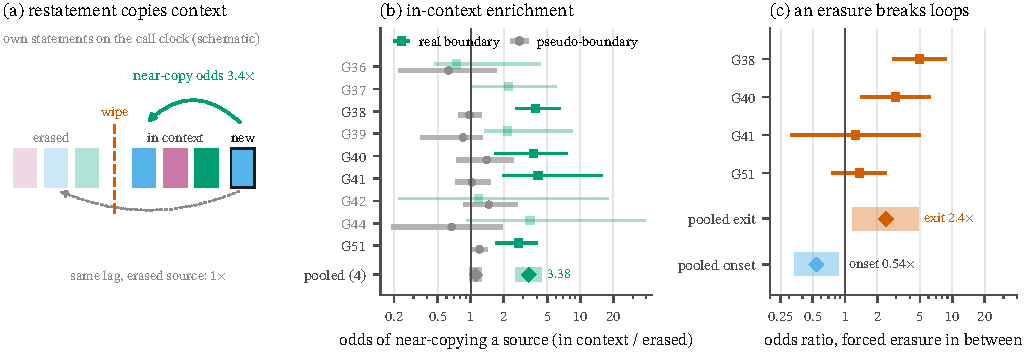
\includegraphics[width=\textwidth]{H69-restatement-loops/fig.pdf}
\caption{Restatement loops copy what is still in the context window. (a) A schematic: an agent's own statements on the call clock; an erasure removes the older ones from its context. (b) The odds that a statement copies an in-context source rather than an erased one, per goal period. The gray fake-boundary null sits near 1, and the pool is 3.38. (c) A forced erasure raises the odds that a loop ends $2.40\times$ and lowers the odds that one starts to $0.54\times$.}
\end{figure}
\begin{figure}[h]
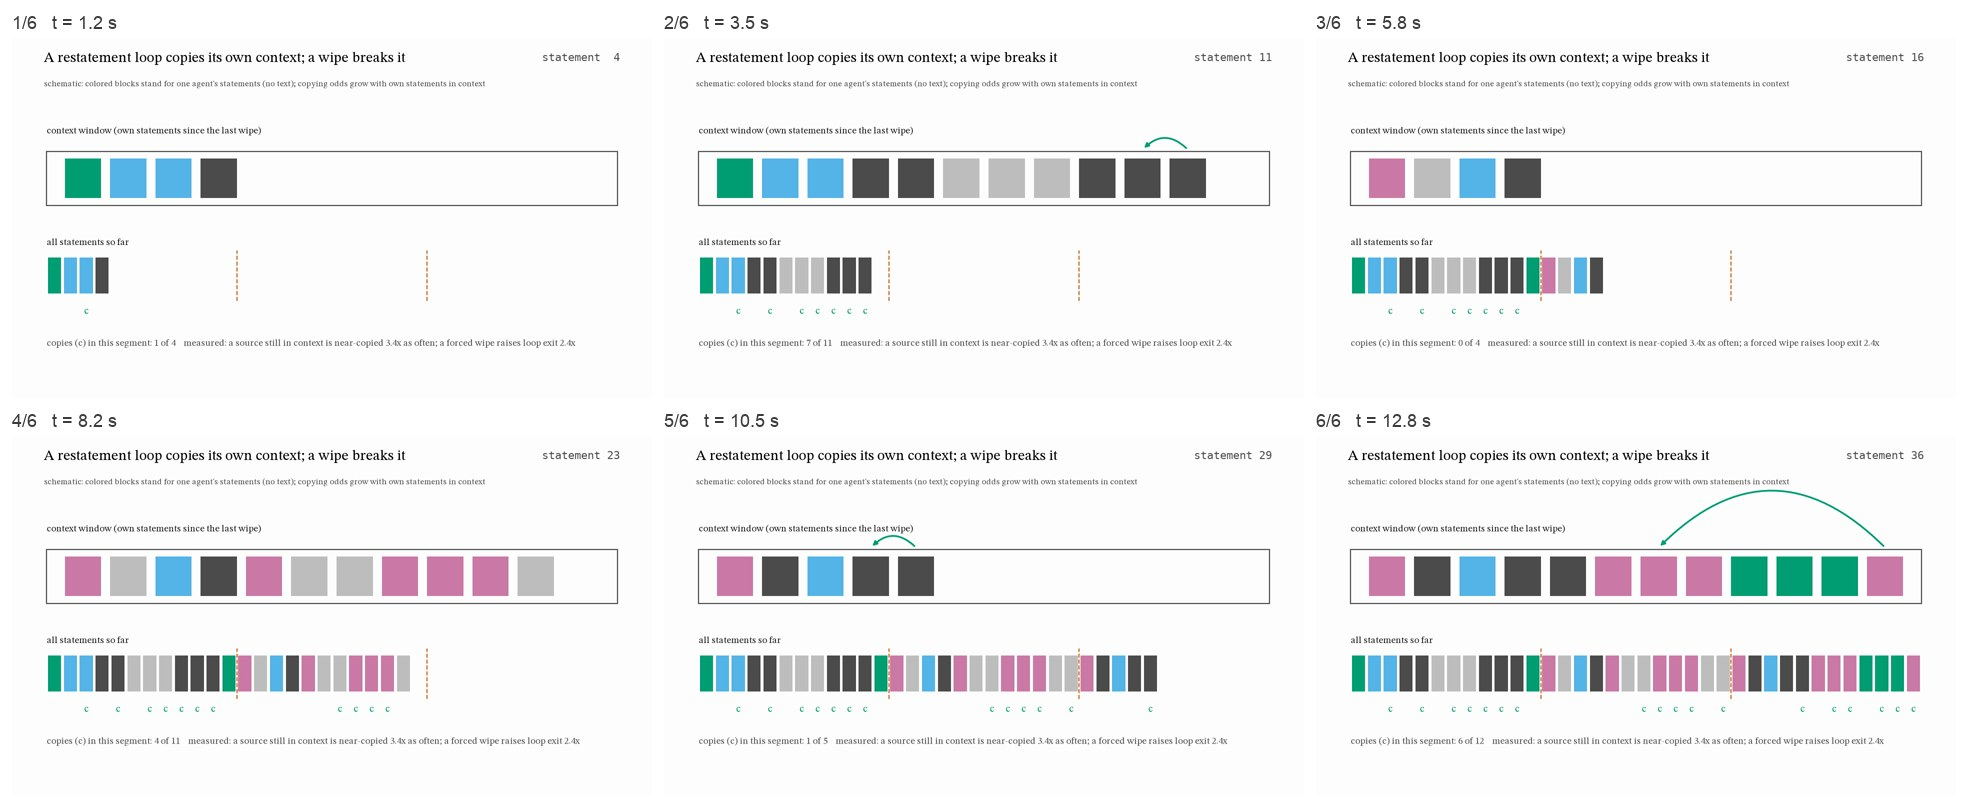
\includegraphics[width=0.9\textwidth]{storyboards/H69.jpg}
\caption{Animation storyboard: six frames of the animation, evenly spaced in time (frame number and time above each). The full animation is \texttt{writeup/animations/H69-restatement-loops.mp4}.}
\end{figure}


\noindent Animation: \texttt{writeup/animations/H69-restatement-loops.mp4}.

\textbf{What it means:} For an operator: to break a restatement loop, erase or trim the agent's context. One forced erasure more than doubles the exit odds and halves the onset odds. Do not rely on messages: nudges read inside a loop do not help (0.81). A busy room does not protect an agent either. For a scaffold builder: cap the agent's own chat kept in context, for example by dropping its oldest self-messages. Each doubling of the agent's own statements in its window raises onset odds by about $\times1.25$. The 41-call cap already acts as a loop breaker, at a cost of 4--10\% of output (H44).

\textbf{Caveats:} Only four periods have at least 30 loop episodes. The erasure exit effect varies across them ($I^2=0.74$; G51 1.36, not significant). The effect size depends on the embedding model. The self-share counts chat items, not the agent's tool output, which dominates prompt tokens. Memory and artifacts may still carry erased statements, so the enrichment is a lower bound. The threshold test (P2) had no power. Context fill also raises onset, which links to H46's style drift. The confirmation script is written and dry-run; no confirmation test on reserved goal periods has run yet.

\section{H05: Rooms couple chat only through reading}
\label{sec:H05}

\textbf{The question:} An agent sees only the chat of its own room. When a split puts two groups in different rooms, does the coupling between the groups vanish while the coupling inside each room holds? Does the swarm's irreversibility (entropy production) fall with it?

\textbf{The intuition:} Treat each agent as a spin: up in a minute when it talks, down when it is silent. A coupling $J_{ij}$ is how much agent $j$'s talk in one minute raises agent $i$'s talk in the next. In this kinetic Ising model, spins update each step in response to a field (here the shared daily schedule) and to their couplings. Room-mates read each other, so the within-room coupling $J_\mathrm{in}$ is positive. A cut removes the cross-room reads, so the cross-room coupling $J_\mathrm{out}$ should fall to zero. The rooms then act as two coupled blocks. Entropy production measures how different the swarm's movie looks when you play it backwards. Asymmetric couplings create it, so a cut should remove its cross-room part.

\begin{figure}[h]
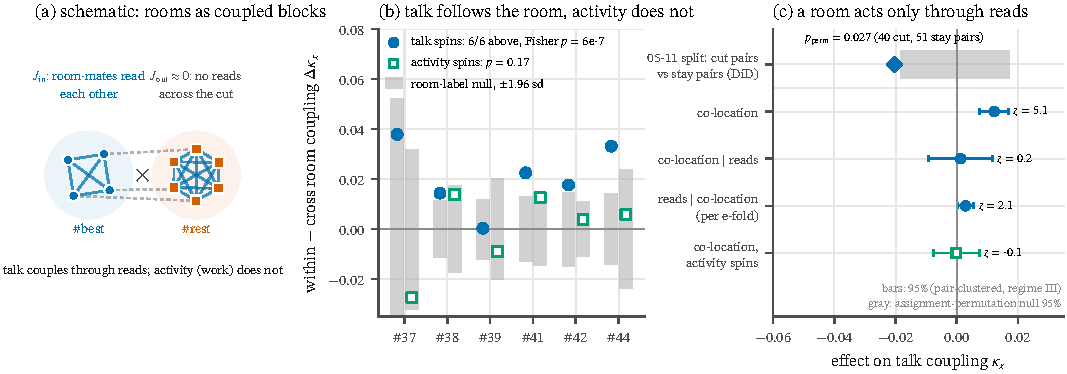
\includegraphics[width=\textwidth]{H05-rooms-cut/fig.pdf}
\caption{Rooms decouple chat only through what agents read. (a) The two-block picture: room-mates read each other, and a cut removes the cross-room reads. (b) Talk coupling follows the room in all six regime-III two-room windows, and activity does not (gray: random room labels). (c) At the 05-11 split, cut pairs lose talk coupling, and the co-location effect disappears once ledger read counts enter the model.}
\label{fig:int-H05}
\end{figure}

\textbf{What we measured:} The observable is the lagged talk coupling $\kappa_x$ of each pair-day, minus a cross-day surrogate. The surrogate pairs agent $i$'s day with another day of agent $j$, aligned by minute, so it keeps the shared schedule and removes interaction. We compared within-room and cross-room pairs against random room labels. We ran pair difference-in-differences (DiD) at room splits, and a panel with pair and day effects. A new test (HH248) added context-ledger read counts to the panel. Impostors: the cross-day surrogate, after a trim to the all-present window, removes the scheduler field. Day effects and goal-change placebos remove most of the external drive, but room-specific kickoffs stay in. The shared model prior is open (no same-family term). Read counts absorb the room effect, but no ``posted but unread'' arm exists, so common input is only partly removed. The synthetic check used kinetic Ising swarms at village sampling. The fitted couplings correlate with the true ones at $r=0.89$--$0.95$, and the pair DiD recovers a planted cut in 20/20 runs. The power for one room event is only 23--63\%.

\textbf{What we found:} Rooms are coupled blocks for talk, and the coupling runs through reading\cred{0.88}; EU 2.2 (value if true 2.5). Within-room talk coupling exceeds cross-room coupling in 6/6 regime-III two-room windows (Fisher $p=6\times10^{-7}$); the per-period rule passes in G38, G41, G42 and G44. Co-location raises $\kappa_x$ by $+0.0123$ ($z=5.1$). With $\log(1+\text{reads})$ in the model, this falls to $+0.0013$ ($z=0.2$), and reads keep $z=2.1$. At the 05-11 split (NE42), cut pairs lose coupling against stay pairs (DiD $-0.020$, $p=0.027$), and stay pairs gain $+0.022$ $[0.013, 0.032]$. Activity spins, the actual work, show no room structure ($p=0.17$). Pairwise entropy production equals the schedule null in 18/18 windows (every $p\ge0.07$). The scope is six windows plus the \#focus cut (G51) and NE42. The summary page says 15/18 for entropy production; we use the card's latest round (the recheck), which gives 18/18.

\textbf{What it means:} For an operator, a room is a read filter. To decouple two agents, stop them reading each other. A room move works only as far as it cuts reads: at \#focus the cross-room reads fell 95\%. Expect co-location to add about 0.01 to the talk coupling, and a split to remove about 0.02. Do not use rooms to divide work, because activity does not follow the room. For a physicist, pairwise entropy production on one-minute spins stays at the schedule null.

\textbf{Caveats:} Co-location and log read counts correlate at 0.82, so the mediation test has little leverage (standard error $\times2.2$). H05 ran one confirmation test on reserved goal periods (NE12/NE15, 2026-10-03), and it was inconclusive. The pair DiD passed ($-0.022$ $[-0.038,-0.008]$, $p=0.021$), the pooled panel missed ($z=1.4$), and $J_\mathrm{in}$ rose about $\times6$ without a prediction. That run used the faulty activity table, which dropped about half of all events, and nobody re-ran it. The \texttt{ep\_gauss\_crossfit} recheck withdrew the \#42 entropy-production exception ($+0.24\to+0.056$, $p=0.10$). The chat result is close to a restatement of the visibility scaffold, and a shared objective confounds the NE42 merge week.

\section{H36: A topic-shift alarm beats a fluctuation alarm}
\label{sec:H36}

\textbf{The question:} Can an operator see from the logs, each day, that the swarm is reorganizing, for example after a goal, room or scaffold change? Do collective fluctuation statistics peak at these transitions, and do they beat a plain topic-shift detector?

\textbf{The intuition:} Near a phase transition, a physical system fluctuates strongly and its parts move together. Flocks show this during a collective turn. We use three statistics. \emph{Susceptibility} is the variance of the swarm's total divided by the sum of the agents' variances; it is 1 for independent agents. The \emph{heat-capacity analogue} is the variance of the alignment energy: how much the agreement between agent pairs swings during a day. \emph{Multi-information} is the total correlation of all agents: how much less random the whole is than its parts. The rival picture says that a goal change is a field step, a new external push between two days. A field step changes where agents point, not how strongly they couple. Fluctuation statistics are then blind to it, but a detector that tracks the mean sees it at once.

\begin{figure}[h]
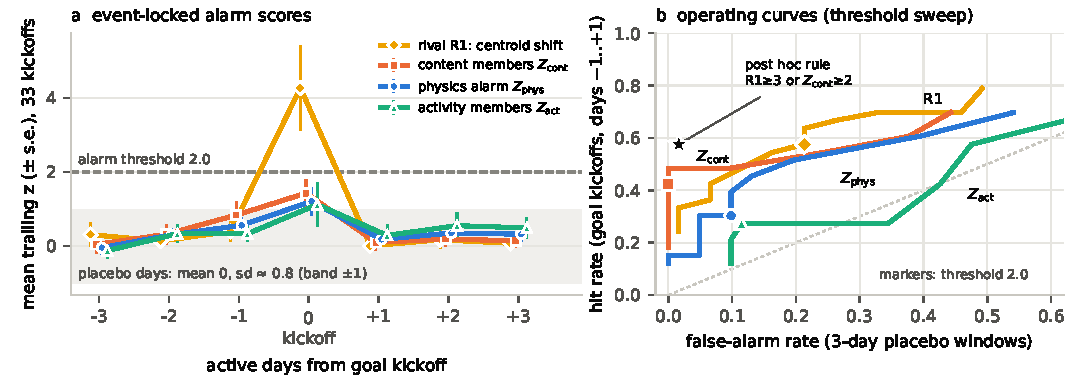
\includegraphics[width=\textwidth]{H36-reorganization-alarm/figures/summary_obs.pdf}
\caption{Fluctuation statistics barely mark goal changes. (a) Mean alarm scores around 33 kickoffs: the physics alarm and its content part rise but stay below threshold, while the topic shift (R1) jumps. (b) Hit rate against placebo false-alarm rate as the threshold changes; the star is the post hoc rule (R1~$\ge$~3 or $Z_\mathrm{cont}\ge2$).}
\label{fig:int-H36}
\end{figure}

\textbf{What we measured:} For each day outside the reserved goal periods (282 days), we computed each statistic as an excess over surrogates shuffled within the day. We used one-minute activity spins, four activity classes and 30-minute content vectors. A trailing 10-day $z$-score feeds the pre-registered alarm $Z_\mathrm{phys}\ge2$. The targets are 33 goal kickoffs. The nulls are placebo days far from every event, Monday placebos and random event dates. The rival R1 is $1-\cos$ between today's and yesterday's mean content vector. Impostors: within-day surrogates, a stall mask and the all-present trim remove the scheduler field. Monday placebos only partly remove the external drive, and about 40\% of the content signal is a drift after the kickoff. The shared model prior is open, because the content vectors carry no style residualization. Common input is not relevant, because the alarm makes no influence claim. In the synthetic check at village sampling, the alarm finds a content-coupling switch (AUC 0.93) but an activity-coupling switch only partly (AUC 0.77). It is blind to field steps at a day boundary, as designed, and R1 catches a goal switch (AUC 1.00).

\textbf{What we found:} Plain topic shift detects goal changes far better than the physics alarm\allowbreak\cred{0.80}; EU 2.2 (value if true 2.75). R1 has AUC 0.95 with the bge embedding and 0.97 with gte. The physics alarm hits 0.27 (bge) or 0.21 (gte) of goal changes at a window false-alarm rate of 0.11. Its AUC is 0.68 $[0.57, 0.79]$ or 0.66 $[0.54, 0.77]$. Against random dates it gives $p=0.08$ or $0.21$, at the pre-registered failure boundary. It loses to R1 by $\Delta$AUC $-0.29$ $[-0.42,-0.17]$ or $-0.34$ $[-0.48,-0.21]$. All of its signal comes from content ($Z_\mathrm{cont}$ AUC 0.74--0.78); the activity channel is at chance (0.50 after the trim). It catches 1/13 scaffold changes, and no score found the undocumented platform steps NE40 and NE45 blind. The scope is the goal changes in goal periods outside the reserved data, plus five native tests (NE38--NE45).

\textbf{What it means:} For an operator, run R1 each day. Raise the alarm when R1 reaches 3 trailing standard deviations, or when the within-day content alignment $Z_\mathrm{cont}$ reaches 2. In-sample, this rule catches 55\% of goal changes at a 2\% window false-alarm rate (bge), or 67\% at 13\% (gte). Do not build the alarm on activity fluctuations, because they follow who is present and how long the day is. For scaffold changes, add log features such as the event mix and tool schemas.

\textbf{Caveats:} The fragile flag is set: the verdict moves with the embedding model and the dedupe rule (bge without dedupe: $p=0.11$). We chose the operator rule post hoc from seven candidates. The test has daily resolution only, with 55 placebo days and none in regime II. Most kickoffs fall on a Monday, and only 11 placebos are Mondays. No confirmation test on reserved goal periods exists yet, and \texttt{confirm.py} must first be re-frozen on the fixed activity table. The alarm on the first nudge-free day (NE43b) is one day with no replication.

\section{H13: Model families share a writing style, not a coupling}
\label{sec:H13}

\textbf{The question:} Do agents from the same lab share a direction in content space beyond the day's goal, a family field? Do same-lab agents couple more strongly with each other than with other labs? Does the family or the room decide who moves with whom?

\textbf{The intuition:} Treat each agent's daily chat as a vector spin, an arrow in a 32-dimensional embedding space. The arrow is a sum: the day's common field (the goal), a family field, the agent's own offset and fluctuations. A field is a fixed push that sets where an arrow points; a coupling makes two arrows move together. A family field has two readings. In the \emph{position} reading, a lab takes its own stance on each period's material, so the field changes with the period. In the \emph{style} reading, the field is a fixed formatting offset that style features remove. Family preference in interaction (homophily) would show as stronger coupling blocks inside each family.

\begin{figure}[h]
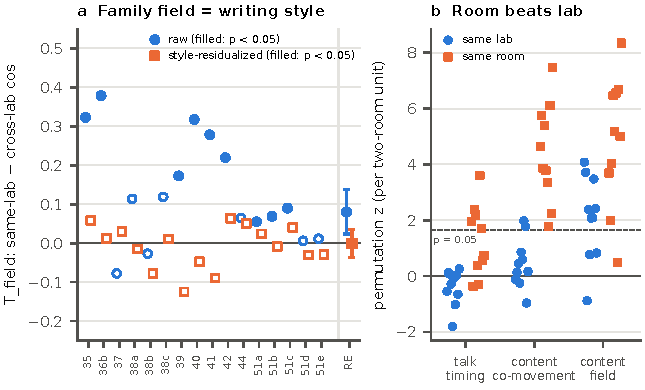
\includegraphics[width=\textwidth]{H13-family-fields/figures/summary_obs.pdf}
\caption{The family field is writing style. (a) The family-field statistic per unit before (blue) and after (orange) the removal of writing-style features; filled markers have permutation $p<0.05$. (b) In two-room units, talk timing and content co-movement follow rooms, not labs.}
\label{fig:int-H13}
\end{figure}

\textbf{What we measured:} The statistic $T_\mathrm{field}$ is the mean cosine between same-lab agents' mean vectors, minus that of cross-lab pairs, after we subtract each day's mean vector. The null shuffles lab labels inside each unit. The style rival regresses each embedding on 20 style features (length, bullets, punctuation, pronouns) and recomputes $T_\mathrm{field}$ on the residuals. For coupling, we fit a block mean field to talk spins and to 30-minute content co-movement, and a pair regression on same-lab and same-room terms. Impostors: a cross-day surrogate partly removes the scheduler field (no all-present trim). Day-mean subtraction removes the external drive. The shared model prior is the object of the card, and two style rivals remove it. Common input is open, because ``rooms carry coupling'' rests on co-movement, not reads. In the synthetic check at village sampling, every test kept its nominal false-positive rate (0.01--0.06). A world with room couplings only did not trigger the family test.

\textbf{What we found:} Model-family content fields are writing style, and behavior carries only a weak family trace\cred{0.87}; EU 2.17 (value if true 2.5). A family field exists in 9/15 units, with random-effects $T=0.080$ $[0.024, 0.137]$ (gte: 8/15, $0.085$). It is stable across periods (split-half cosine 0.88 against a null of 0.76, $p\le0.008$). After style residualization, it survives in 0/9 units ($T=-0.001$ $[-0.037, 0.035]$), and the 20 style features alone identify labs in 14/15 units. Families do not couple by family: the contrast is $-0.003$ $[-0.021, 0.016]$ in talk timing and $-0.002$ $[-0.019, 0.015]$ in content co-movement. Rooms carry the coupling: for co-movement the room term is $0.217$ $[0.163, 0.271]$ and the lab term $0.013$. A behavioral family field fails its rule (3/15 units, $0.075$ $[0.030, 0.121]$); it lives mostly in file-write and commit cadence. The scope is 15 units in \#35--\#44 and \#51, with natives NE06, NE32 and G35.

\textbf{What it means:} Any consensus or alignment metric built on embeddings must remove writing style first. Without style control, labs look like blocs in 9/15 units; with it, in 0 of those 9. Do not infer a vendor ``ideology'' or collusion from content. To control who interacts, use rooms: their term is about $17\times$ the lab term. To fingerprint a lab, use the 20 style features.

\textbf{Caveats:} The no-coupling results exclude only couplings of about 0.1 (talk) or 0.08 (content) and above. The style rival is the strongest possible; a gentler one keeps a third of the field in 4/15 units, so ``only style'' is not shown. The day-mean subtraction weakens Anthropic's field (about 40\% of agents). The behavioral field can come from each provider's tool conventions, and NE06 hit every agent, so it cannot separate the two. Newcomers match their lab in 4/11 cases by content ($p=0.06$). No confirmation test on reserved goal periods has run.

\section{H67: The talk loop sits far below runaway}
\label{sec:H67}

\textbf{The question:} When one agent posts a message, how many extra messages does it cause through other agents reading it? Is this loop gain close to 1, where talk cascades run away? Does a dial on the read-out call see more gain than the one-minute equal-time dial of H25?

\textbf{The intuition:} Think of a microphone near a speaker. Each sound comes back multiplied by the loop gain $g$. If $g<1$, a push dies out, and the total amplification is $\chi=1/(1-g)$. At $g=1$ the system howls; this is the critical point. In a branching process, $g$ is the mean number of offspring of one event. Here the offspring are talk messages that reading causes. The scaffold lets an agent read new messages only at its next model call, the read-out call. So the response should appear at that call. The equal-time dial counts co-movement inside one minute. It can therefore mistake a shared field (all agents reacting to the same burst or schedule) for coupling.

\begin{figure}[h]
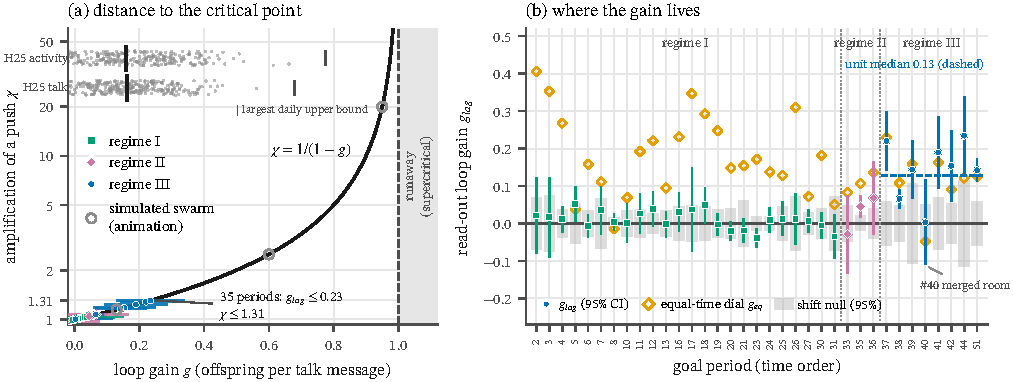
\includegraphics[width=\textwidth]{H67-subcritical-dial/fig.pdf}
\caption{The talk loop sits far below its critical point. (a) The amplification $\chi=1/(1-g)$ against the loop gain, with every goal period at its read-out gain; no period passes 0.23, against a divergence at 1. (b) The read-out gain per period in time order: about 0 in regimes I and II and about 0.13 in regime III, with the equal-time dial (orange) reading higher from shared fields. Animation: \texttt{writeup/animations/H67-subcritical-dial.mp4}.}
\label{fig:int-H67}
\end{figure}
\begin{figure}[h]
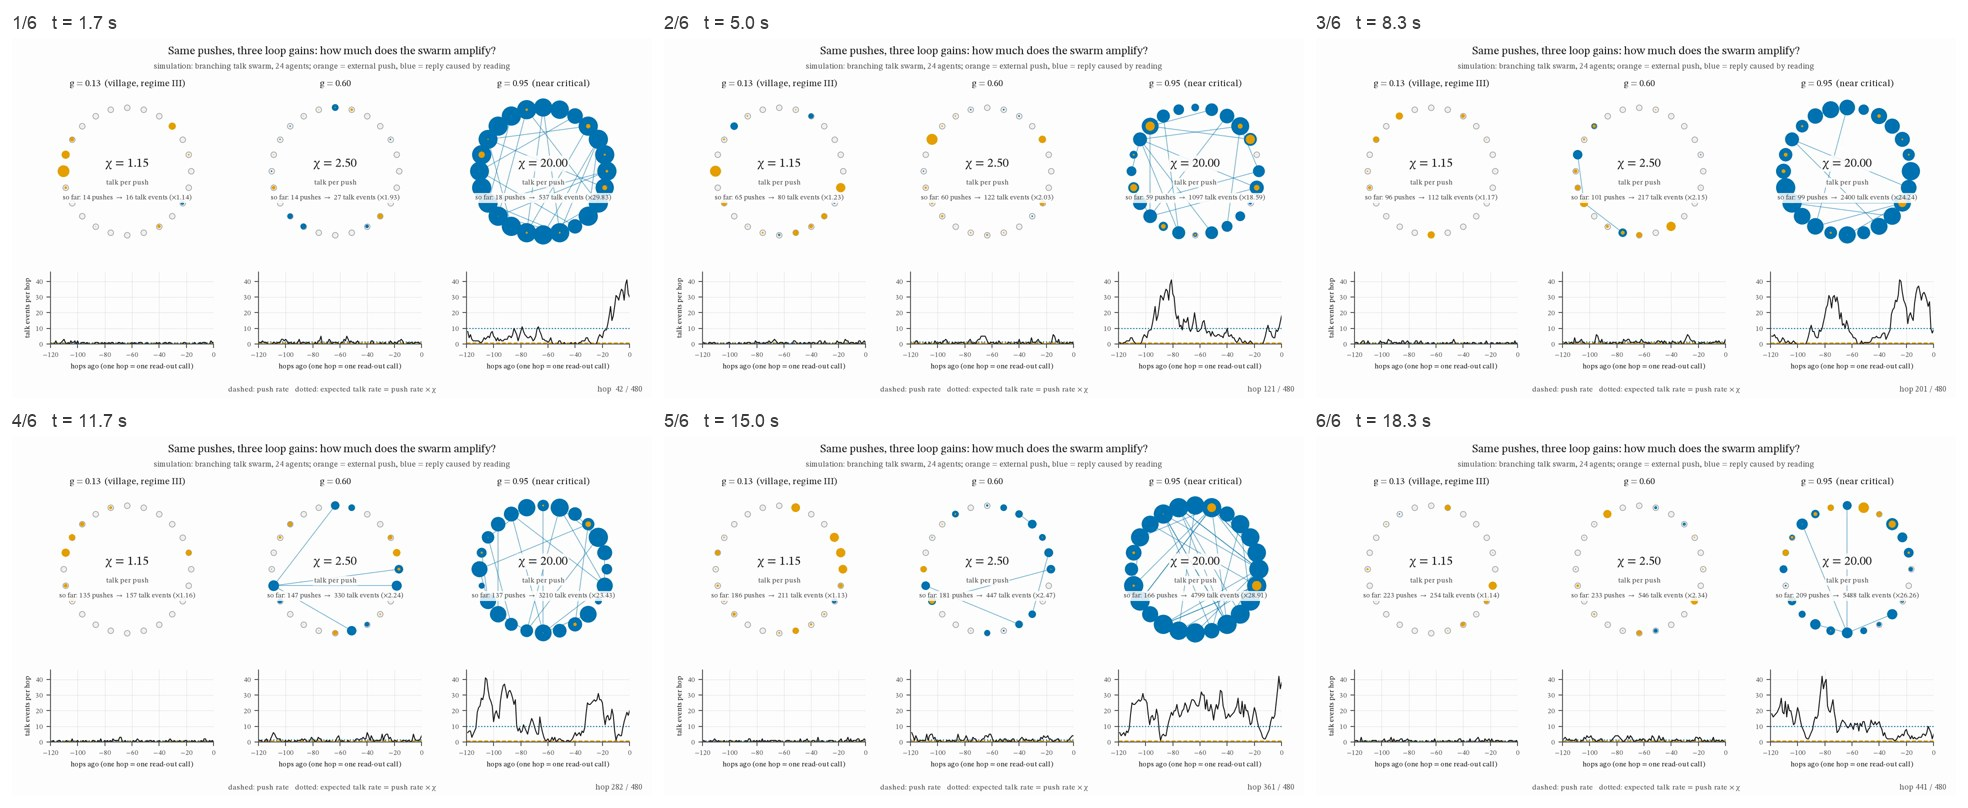
\includegraphics[width=0.9\textwidth]{storyboards/H67.jpg}
\caption{Animation storyboard: six frames of the animation, evenly spaced in time (frame number and time above each). The full animation is \texttt{writeup/animations/H67-subcritical-dial.mp4}.}
\end{figure}


\textbf{What we measured:} The read-out jump $J_1^*$ is the extra talk probability per peer message read at a call. We subtract the effect of messages posted while the call was running (the in-flight placebo, at matched lag). Those messages share every local field, but the call cannot read them. The loop gain is $g_\mathrm{lag}=\bar m\,\bar r\,J_1^*$: messages per talk call times readers per message times the jump. We fit it within each of 66 units in 35 goal periods, on 1.47M receiving calls inside all-present windows.
Impostors: all four are removed. \emph{Scheduler field:} each call is one update with agent $\times$ day $\times$ call-class baselines. The placebo cancels any field that is smooth over one call latency (5--60\,s). \emph{External drive:} human messages and nudges are covariates, and the placebo shares any kickoff burst. \emph{Shared model prior:} agent $\times$ day baselines absorb each agent's talk rate, so only timing identifies the coupling. \emph{Common input:} the in-flight placebo is exactly the ``posted but not yet read'' control.
The synthetic check ran on the real call grids. Planted gains of 0.15--0.60 came back with bias $-1\%$ to $-3\%$ and interval coverage 0.88--0.98. A world with fields only gave $-0.010$. A burst world gave $-0.03$, where the uncorrected gain reads $+0.06$.

\textbf{What we found:} The read-out loop gain of talk is subcritical in 66/66 units\cred{0.79}; EU 2.17 (value if true 2.75). Every unit's upper bound is below 0.40. The regime-III median is 0.13, and \#51 gives $0.142$ $[0.111, 0.174]$. Regime I gives 0.005. The largest goal-period gain is 0.234, so $\chi\le1.31$. At the median, $\chi\approx1.15$ and $T/T_c\approx8$: the swarm runs eight times hotter than its critical point. The coupling acts mostly on named messages. A named message raises the recipient's talk probability by $0.079$ $[0.069, 0.089]$ per read; an unnamed one by $0.004$ $[0.003, 0.006]$ ($\times19$). Named messages give about half of the gain. In \#51 the gain stays flat (0.14) as the swarm grows from 21 to 32 agents. The per-read jump falls with headcount ($\rho=-0.59$). The gain ranks periods like H42's read-out Hawkes fit ($\rho=0.55$, $p=0.0007$). The original claim (lagged gain $>$ equal-time dial) fails: it holds in only 7/35 periods. The equal-time dial reads 0.10--0.31 from fields alone.
The scope is 66 units in 35 goal periods, with the native tests NE14, NE42 and G51.

\textbf{What it means:} For a monitor, report $g_\mathrm{lag}$, not the equal-time dial, as the distance to runaway talk. Expect a push to grow by at most $\times1.31$. No village configuration from 4 to 32 agents came near runaway, so this is a gauge, not a lever. For an operator who wants a reply, name the recipient: that raises its next-call talk probability by 0.08 instead of 0.004. For a scaffold builder, more agents do not push the swarm toward criticality, because each read counts for less.

\textbf{Caveats:} Only the first hop has a placebo correction. Hops 2--3 (median 0.28) have none. Regime-I talk happens at scheduled chat calls, so this estimator uses the wrong clock there. A post hoc subset of quiet recipients lowers the regime-III median to 0.086 ($-34\%$). The unnamed part sits at the resolution of the placebo (bias about $\pm0.03$ in $g$). The shift null rejects in 13.6\% of units (synthetic 7.5--10\%), so single-unit significance is slightly optimistic. H50's estimator gives about twice this gain ($\rho=0.24$). The predictions were written with H25, H42 and H50 known. No confirmation test on reserved goal periods has run.

\section{H16: Idle traps deepen with time}
\label{sec:H16}

\textbf{The question:} Agents sometimes get stuck in long silences, chains of timer pauses or repeated failures. Is the escape from such a trap memoryless, as Kramers escape predicts, or does the trap deepen with time? What gets a stuck agent out?

\textbf{The intuition:} In the Kramers picture, noise kicks a particle over the barrier of its well. It escapes at a constant rate, whatever time it has already spent there: the escape is memoryless. In the aging picture (a Bouchaud trap model), trap depths have a broad spread. The longer an agent stays stuck, the more likely it sits in a deep trap. The hazard, the chance of escape per unit time for an agent still stuck, then falls with time. A kick is a message to the agent. In Kramers, each kick lowers the barrier, so escape rises exponentially with the number of kicks. In the rival picture, the agent reads the kick at its next call, so the first kick does the work and more kicks add little.

\begin{figure}[h]
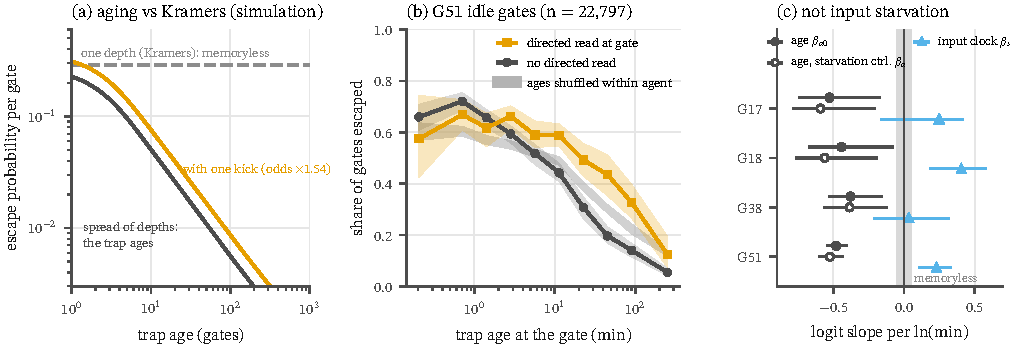
\includegraphics[width=\textwidth]{H16-trap-aging/fig.pdf}
\caption{Idle traps age by themselves, and one directed kick helps. (a) Simulation: with one trap depth the escape chance does not depend on trap age, but with a broad spread of depths it falls. (b) In \#51, fewer pause points start a run of activity as the trap ages, with a directed message (orange) or without one (dark). (c) Aging slopes in four goal periods stay negative when an input-starvation clock enters the model. Animation: \texttt{writeup/visuals/H16-trap-aging/anim.mp4}.}
\label{fig:int-H16}
\end{figure}
\begin{figure}[h]
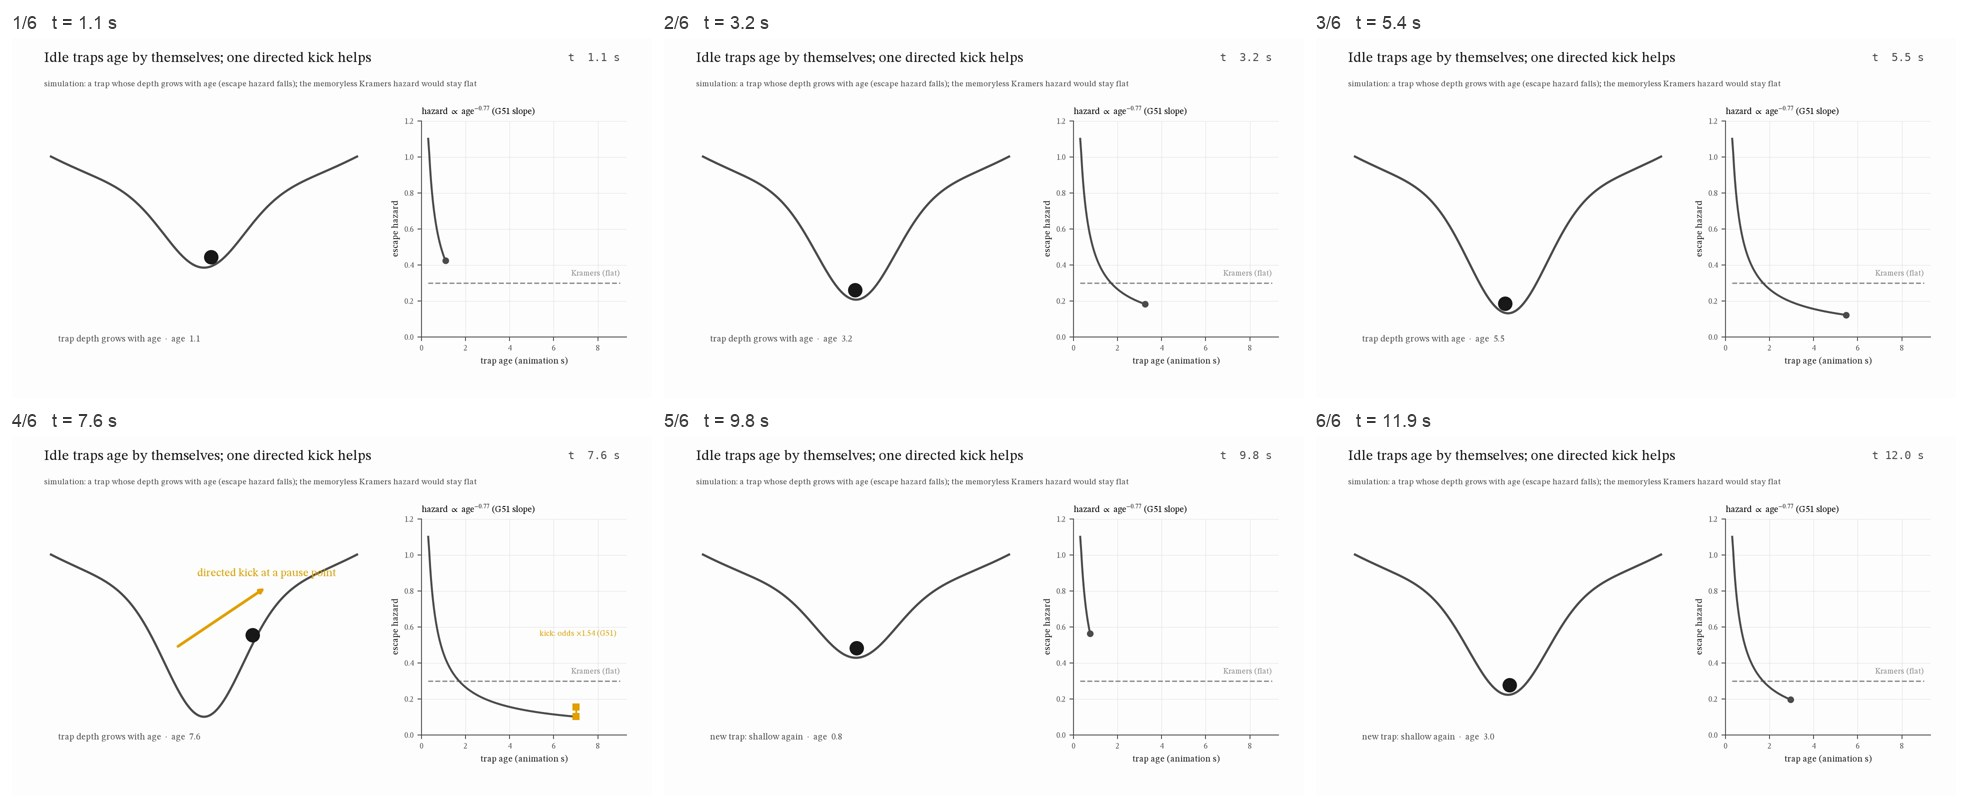
\includegraphics[width=0.9\textwidth]{storyboards/H16.jpg}
\caption{Animation storyboard: six frames of the animation, evenly spaced in time (frame number and time above each). The full animation is \texttt{writeup/visuals/H16-trap-aging/anim.mp4}.}
\end{figure}


\textbf{What we measured:} Inactive spells are gaps of 180\,s or more; single isolated actions do not end them. Pause chains are runs of timer pauses, with one decision at each timer wake. The hazard slope $\beta$ on $\ln(\text{time elapsed})$ uses spells of 10\,min or more, with agent fixed effects: $\beta=0$ is memoryless, $\beta<0$ is aging, and $|\beta|\le0.3$ counts as memoryless. At each timer wake, a logit relates the chance to act to the chain length. A kick is a directed message in the prior 2\,min; the null takes the same agent's kicks from another day. Impostors: agent fixed effects and the day-swap null partly remove the scheduler field. Past-only kicks remove the external drive, and the aging persists with the nudger off (NE43). The shared model prior is not relevant: fixed effects absorb each agent's frailty, and the card makes no family claim. Common input is open, because kicks count by posting time, not by the read-out call. The synthetic check used overdamped Langevin agents seen through event times. Memoryless truth gave $+0.05\pm0.07$; deepening traps gave $-0.58$ and $-1.08$ (truth $-0.54$, $-1.18$). Without fixed effects, frailty alone faked aging of $-0.25$.

\textbf{What we found:} Within an agent, escape from inactive spells and pause chains ages instead of being memoryless\cred{0.70}; EU 2.1 (value if true 3.0). The inactive-spell slope is $-0.77$ $[-0.81,-0.73]$ in \#51 (4,321 escapes) and $-1.71$ in \#38. It is below $-0.3$ in 6/8 regime-III goal periods, but its interval lies below $-0.3$ in only 3/8. The chance to act at a timer wake falls with chain length in 6/7 periods (\#51 $-0.38$). With the nudger off (NE43), the aging does not change ($-0.59\to-0.53$). One directed message during a pause raises the odds of acting at the next timer wake $\times1.5$--$2.9$ in 5/7 periods (\#51 $\times1.54$). The dose response is additive or saturating in 14/16 powered cells, not exponential. On real failures, error-loop aging survives only in \#51 ($-0.57$), and messages do not break failure loops (9/9 periods). The mean-field coupling $\beta J_0$ is 0.09--0.41, so the swarm has no collective bistability. The scope is 11 goal periods (8 in regime III), silences and pause chains only. The credence comes from an adjudication: the coordinator gave a wider claim 0.44 and marked it fragile; the blind rater's 0.70 stood, not fragile.

\textbf{What it means:} For an operator, kick a stuck agent early, because its escape hazard falls roughly as $t^{-0.8}$. Send one directed message during a pause. Under the 5-min pause default, it lifts escape from deep pause chains from 0.17 to 0.25; before that default (NE44), from 0.21 to 0.56. A second message adds little. For an agent in a real failure loop, use tooling or a reset, not messages.

\textbf{Caveats:} Spells of different kinds within one agent can mimic aging, and fixed effects remove only differences between agents. The pre-registered count rule (5/8 periods) is not met, and short periods give unstable bootstrap intervals. The predicted drop in the chance to act with the nudger off failed ($+0.006$ $[-0.09, 0.10]$), and so did the NE44 interaction as stated. We defined the robust pause-chain rule after we saw the data. No confirmation test on reserved goal periods has run. Figure panels (b) and (c) use H72's estimator, whose \#51 aging slope is $-0.48$, not $-0.77$.

\end{document}
